\appendix

\section{CodeQL query} \label{appendix:codeql-query}

\renewcommand\theFancyVerbLine{\footnotesize\arabic{FancyVerbLine}}
\newenvironment{code}{\captionsetup{type=listing}}{}

\begin{code}
    \begin{minted}[linenos=true, tabsize=4, breaklines=true, fontsize=\footnotesize]{python3}
import cpp
import semmle.code.cpp.dataflow.DataFlow
import semmle.code.cpp.security.Overflow
import semmle.code.cpp.metrics.MetricFunction
import semmle.code.cpp.Print

predicate goodFile(MetricFunction mf) {
    not (
        mf.getFile().getAbsolutePath().toString().regexpMatch(".*.pb.cc") or
        mf.getFile().getAbsolutePath().toString().regexpMatch(".*.pb.h") or
        mf.getFile().getAbsolutePath().toString().regexpMatch(".*variant.h") or
        mf.getFile().getAbsolutePath().toString().regexpMatch(".*third_party.*") or
        mf.getFile().getAbsolutePath().toString().regexpMatch("/usr/include/.*") or
        mf.getFile().getAbsolutePath().toString().regexpMatch("/usr/lib/.*") or
        mf.getFile().getAbsolutePath().toString().regexpMatch(".*TypeCast.h") or
        mf.getFile().getAbsolutePath().toString().regexpMatch(".*/ATen/cpu/vec/.*")
    )
}

predicate libfuzzerFuzzable(MetricFunction mf) {
    mf.getNumberOfParameters() = 2 and
    mf.getAParameter().getUnderlyingType() instanceof IntegralType and
    exists(PointerType ptr |
        ptr = mf.getAParameter().getUnderlyingType() and
        ptr.getUnderlyingType().getName().regexpMatch(".*(char|int|byte|void)+.*")
    )
}

int getComplexity(MetricFunction mf) {
    result = mf.getCyclomaticComplexity()
}

predicate goodName(MetricFunction mf) {
    not (
        mf.getName().regexpMatch(".*parallel_for.*") or
        mf.getName().regexpMatch(".*_PlacementNew.*") or
        mf.getName().regexpMatch(".*_PlacementDelete.*") or
        mf.getName().regexpMatch("xnn_.*") or
        mf.getName().regexpMatch("Sleef_.*") or
        mf.getName().regexpMatch("_M_.*")
    )
}

from MetricFunction mf, int cc
where
    cc = getComplexity(mf) and
    goodFile(mf) and
    goodName(mf) and
    libfuzzerFuzzable(mf)
select "Complexity: ", cc, "Function: ", mf, "Declaration", mf.getFullSignature(), "File: ",
    mf.getFile() order by cc desc
\end{minted}
    \caption{CodeQL query used to find fuzzable functions in PyTorch.}
\end{code}

\section{Fuzzbench results} \label{appendix:fuzzbench-results}

\begin{figure}[b]
    \centering
    \resizebox{\columnwidth}{!}{%
        \begin{tabular}{cc}
            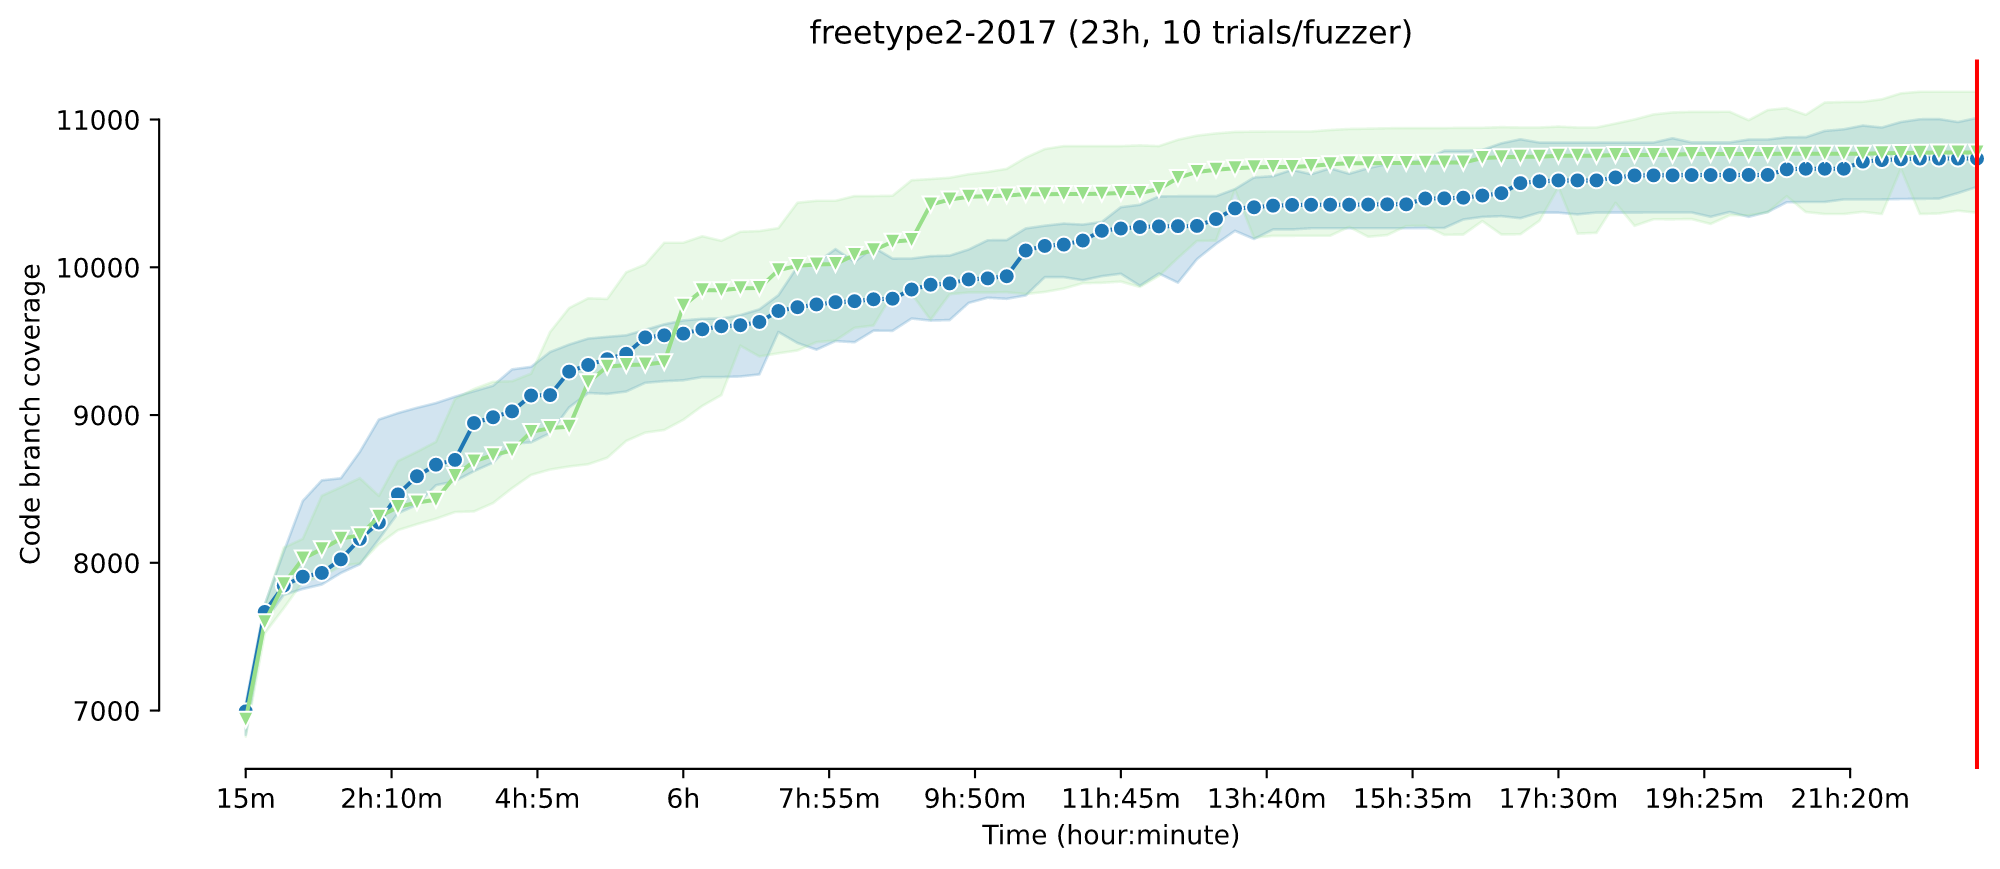
\includegraphics[width=0.65\textwidth]{assets/fuzzbench/symptr-15-1/freetype2-2017_coverage_growth.png}  & 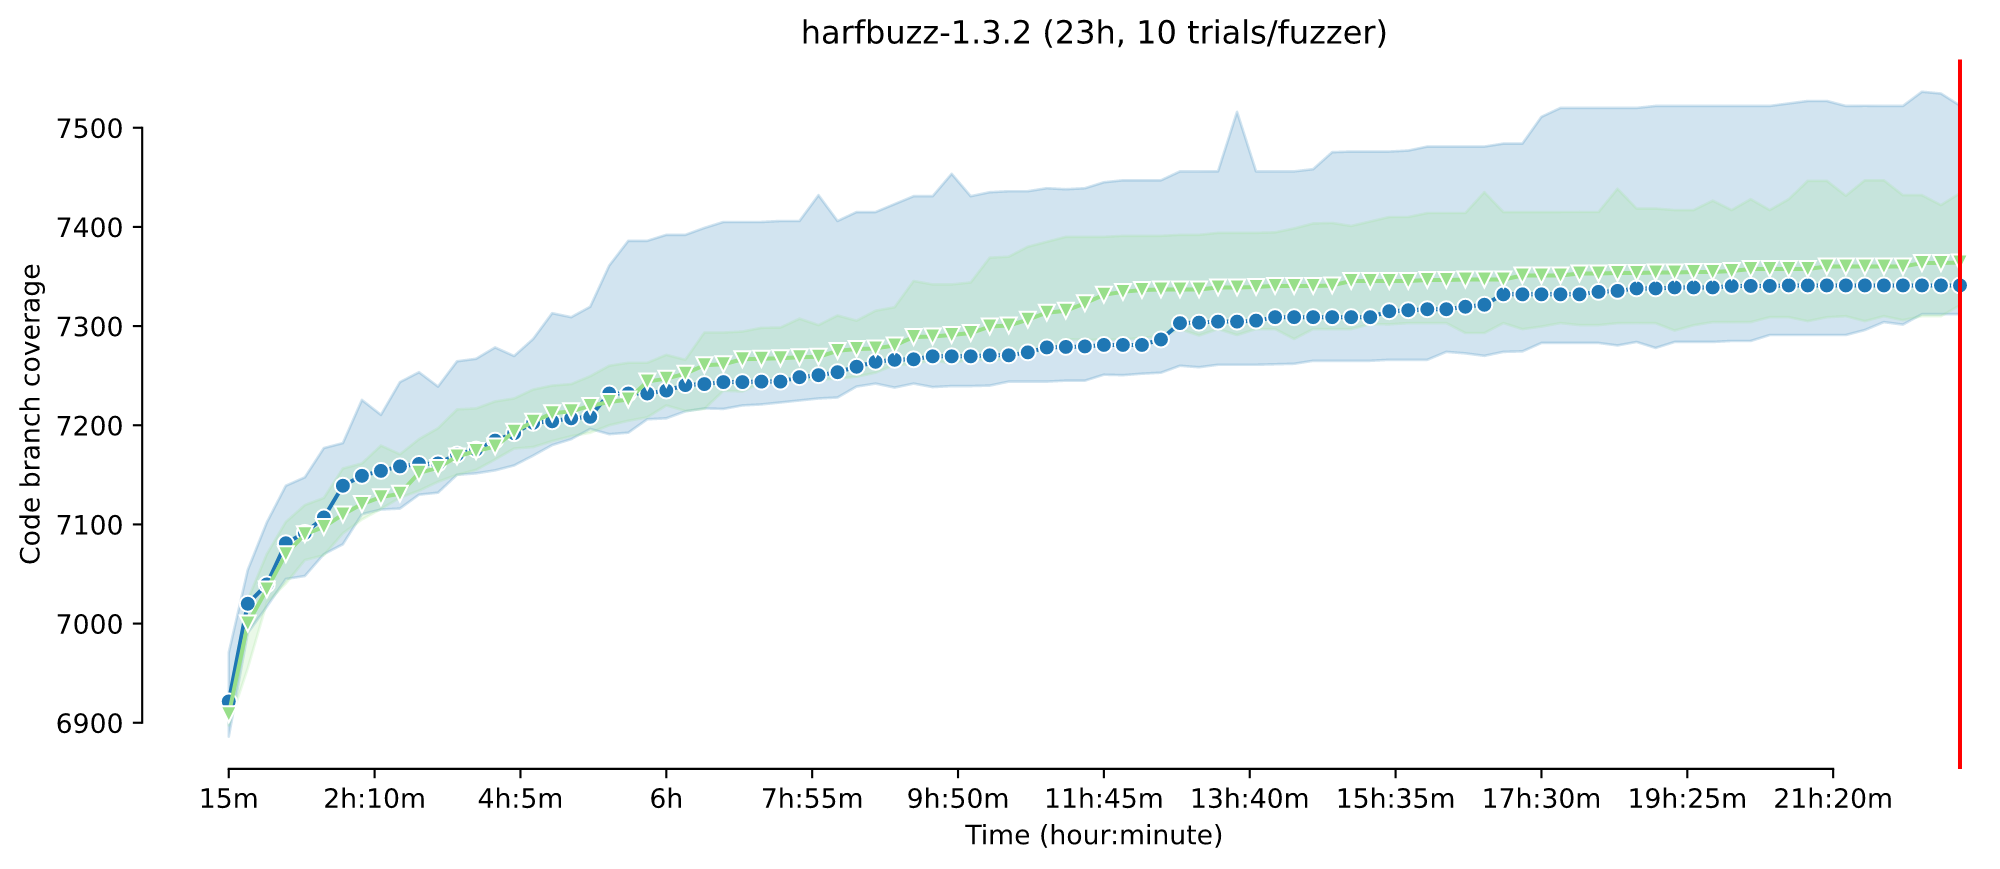
\includegraphics[width=0.65\textwidth]{assets/fuzzbench/symptr-15-1/harfbuzz-1.3.2_coverage_growth.png}        \\
            (a) freetype2                                                                                            & (b) harfbuzz                                                                                                   \\[6pt]
            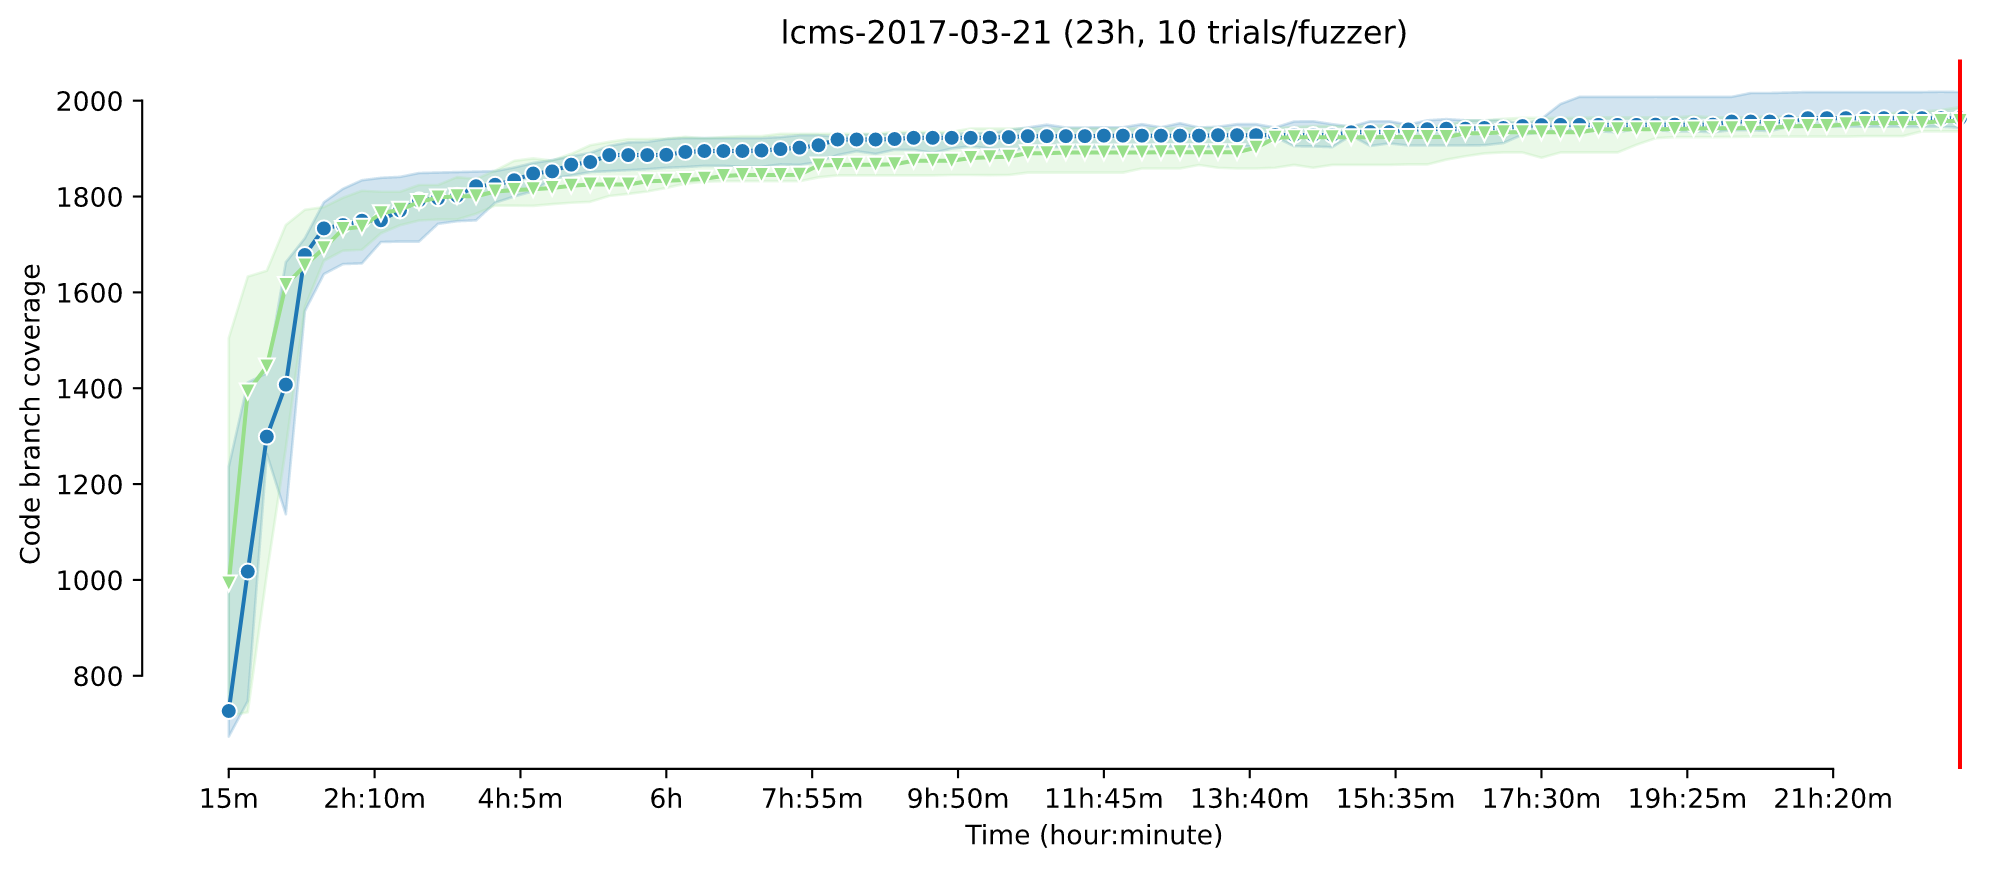
\includegraphics[width=0.65\textwidth]{assets/fuzzbench/symptr-15-1/lcms-2017-03-21_coverage_growth.png} & 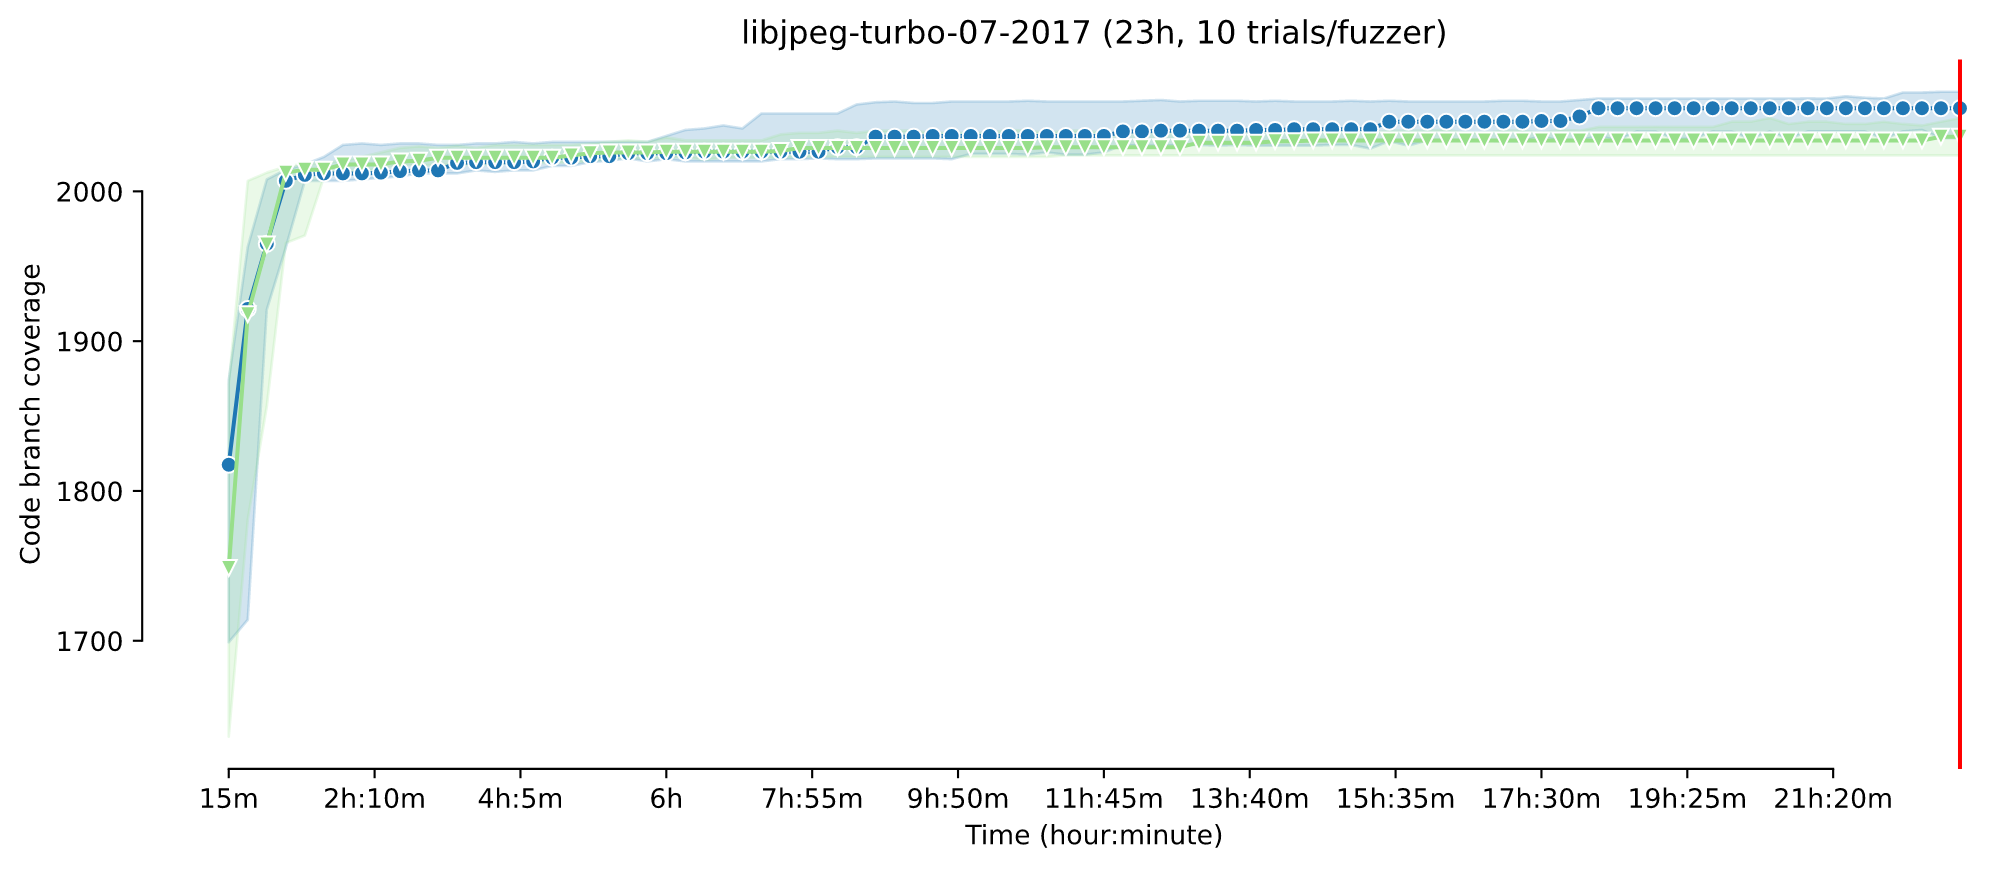
\includegraphics[width=0.65\textwidth]{assets/fuzzbench/symptr-15-1/libjpeg-turbo-07-2017_coverage_growth.png} \\
            (c) lcms                                                                                                 & (d) libjpeg                                                                                                    \\[6pt]
            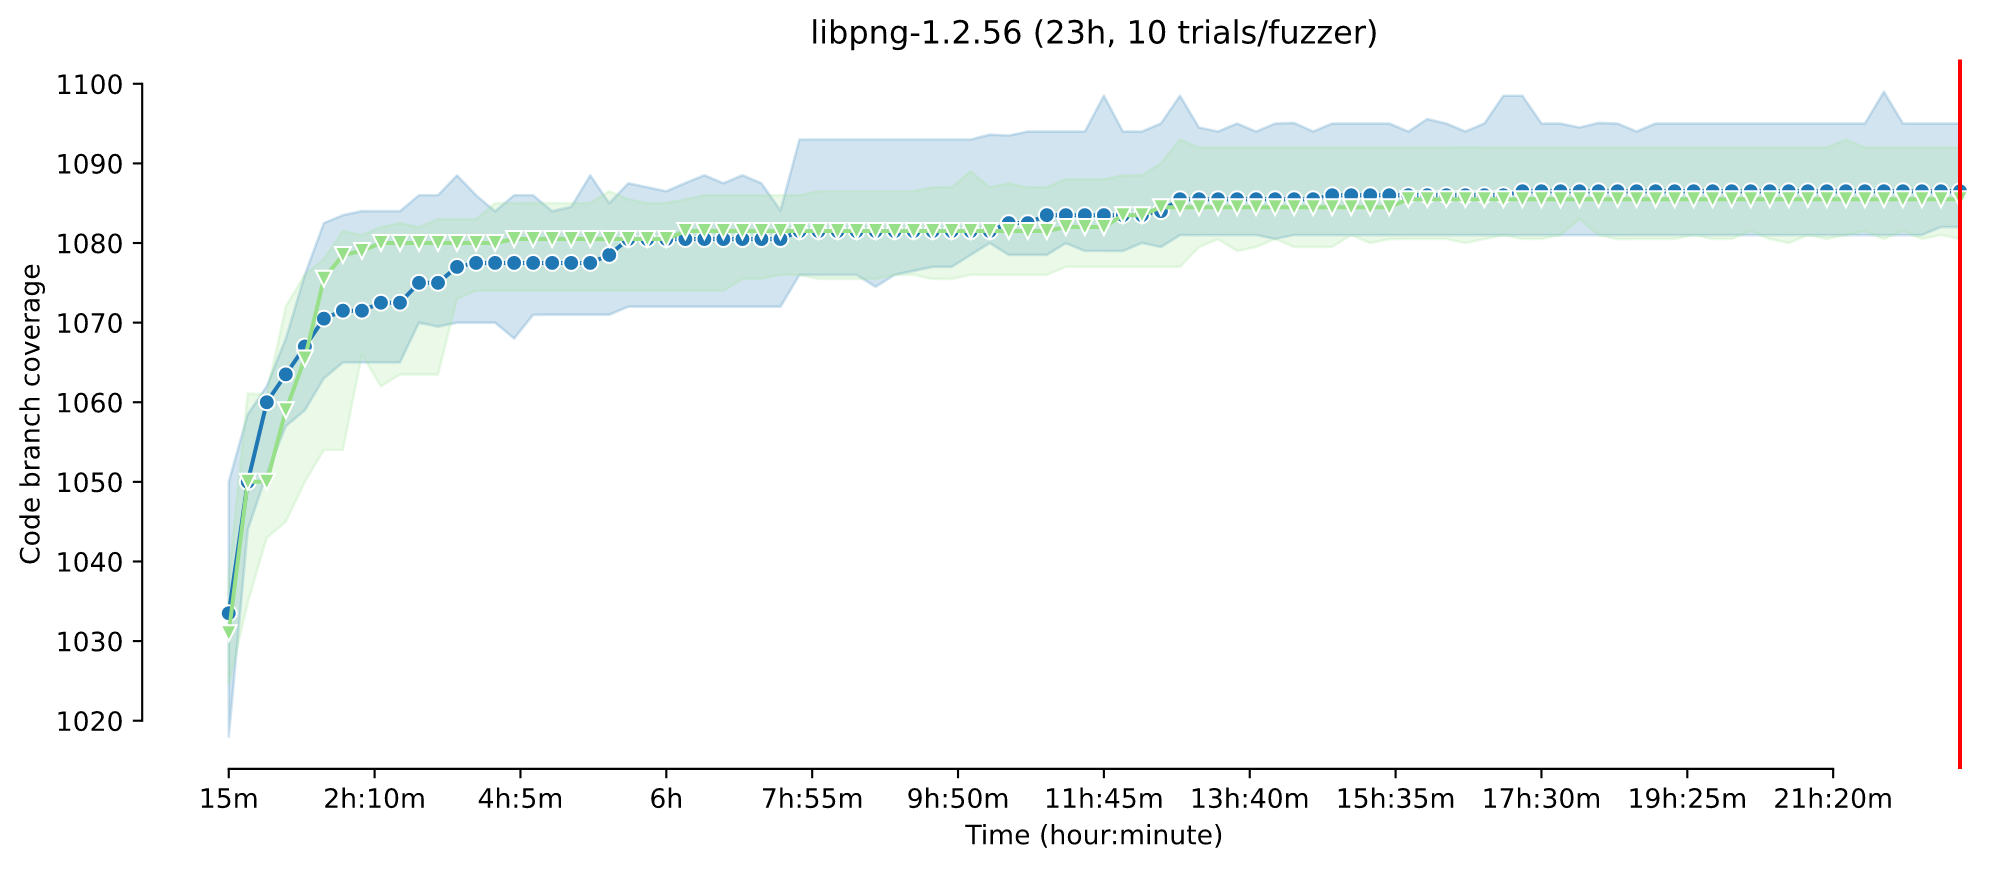
\includegraphics[width=0.65\textwidth]{assets/fuzzbench/symptr-15-1/libpng-1.2.56_coverage_growth.png}   & 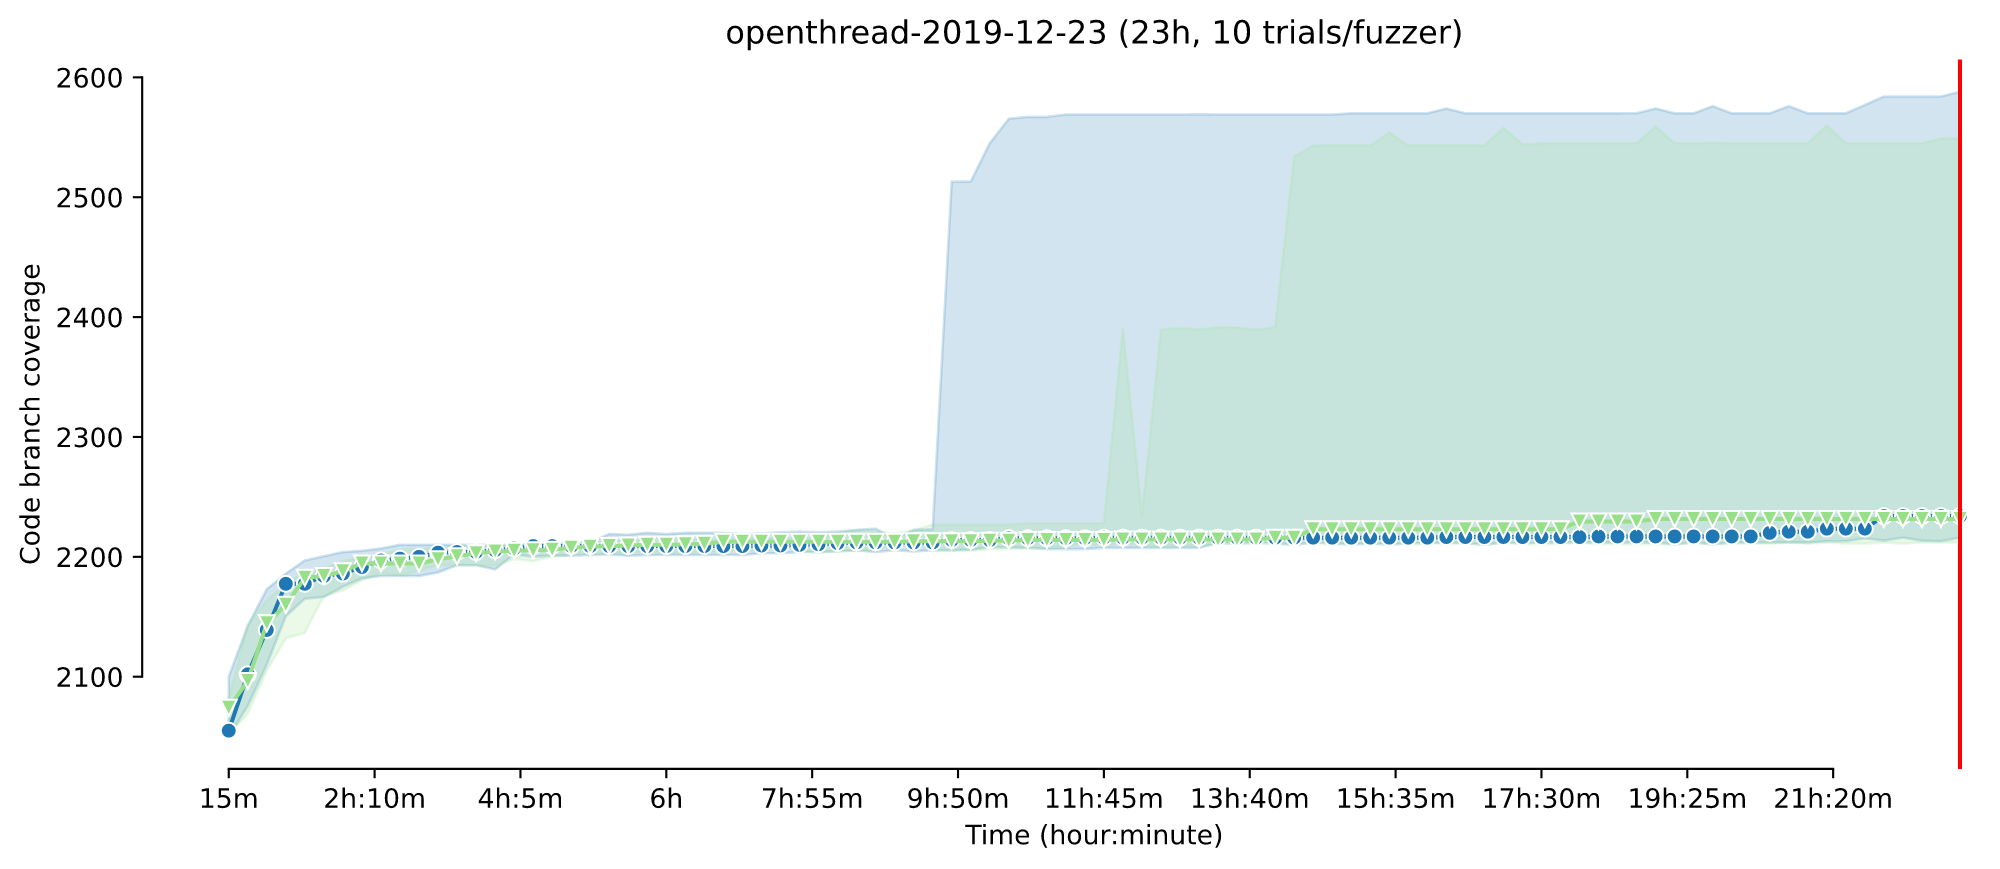
\includegraphics[width=0.65\textwidth]{assets/fuzzbench/symptr-15-1/openthread-2019-12-23_coverage_growth.png} \\
            (c) libpng                                                                                               & (d) openthread                                                                                                 \\[6pt]
            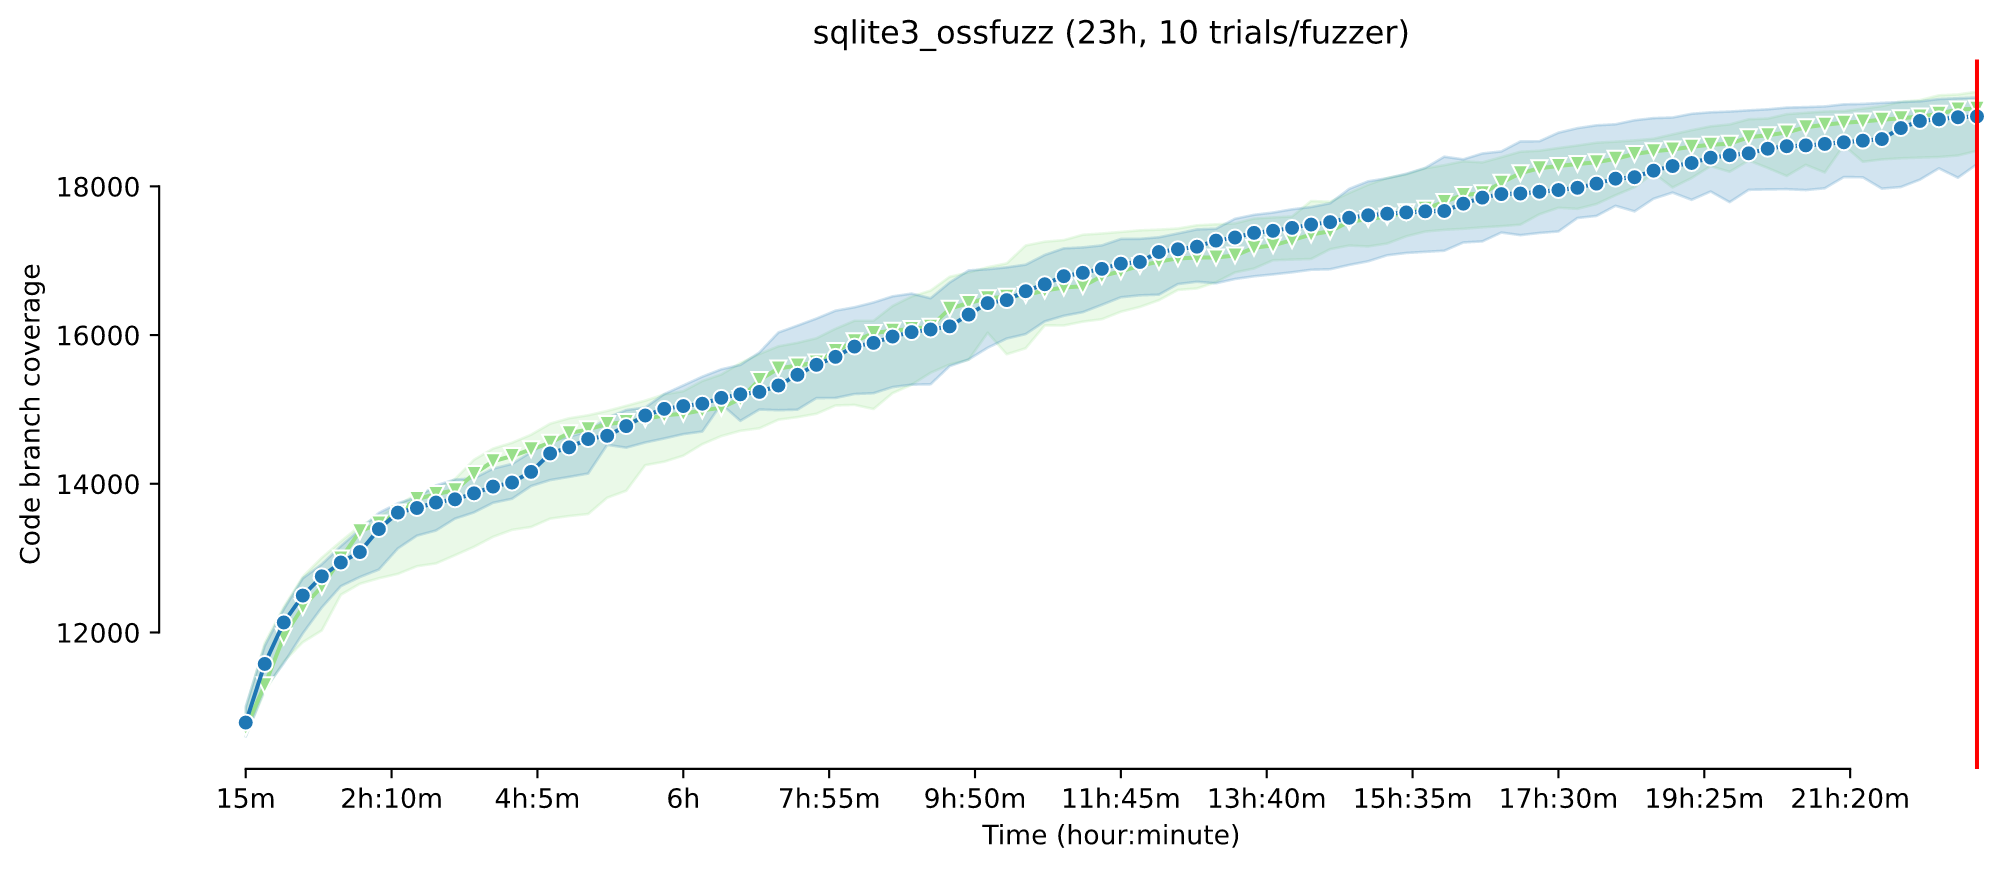
\includegraphics[width=0.65\textwidth]{assets/fuzzbench/symptr-15-1/sqlite3_ossfuzz_coverage_growth.png} & \includegraphics[width=0.65\textwidth]{assets/fuzzbench/symptr-15-1/fuzzbench-legend.png}                      \\
            (c) sqlite3                                                                                              & (d) legend                                                                                                     \\[6pt]
        \end{tabular}
    }
    \caption{Fuzzbench: Symptr-15-1 coverage growth.}
    \label{fig:fuzzbench:symptr-15-1}
\end{figure}

\begin{figure}[b]
    \centering
    \resizebox{\columnwidth}{!}{%
        \begin{tabular}{cc}
            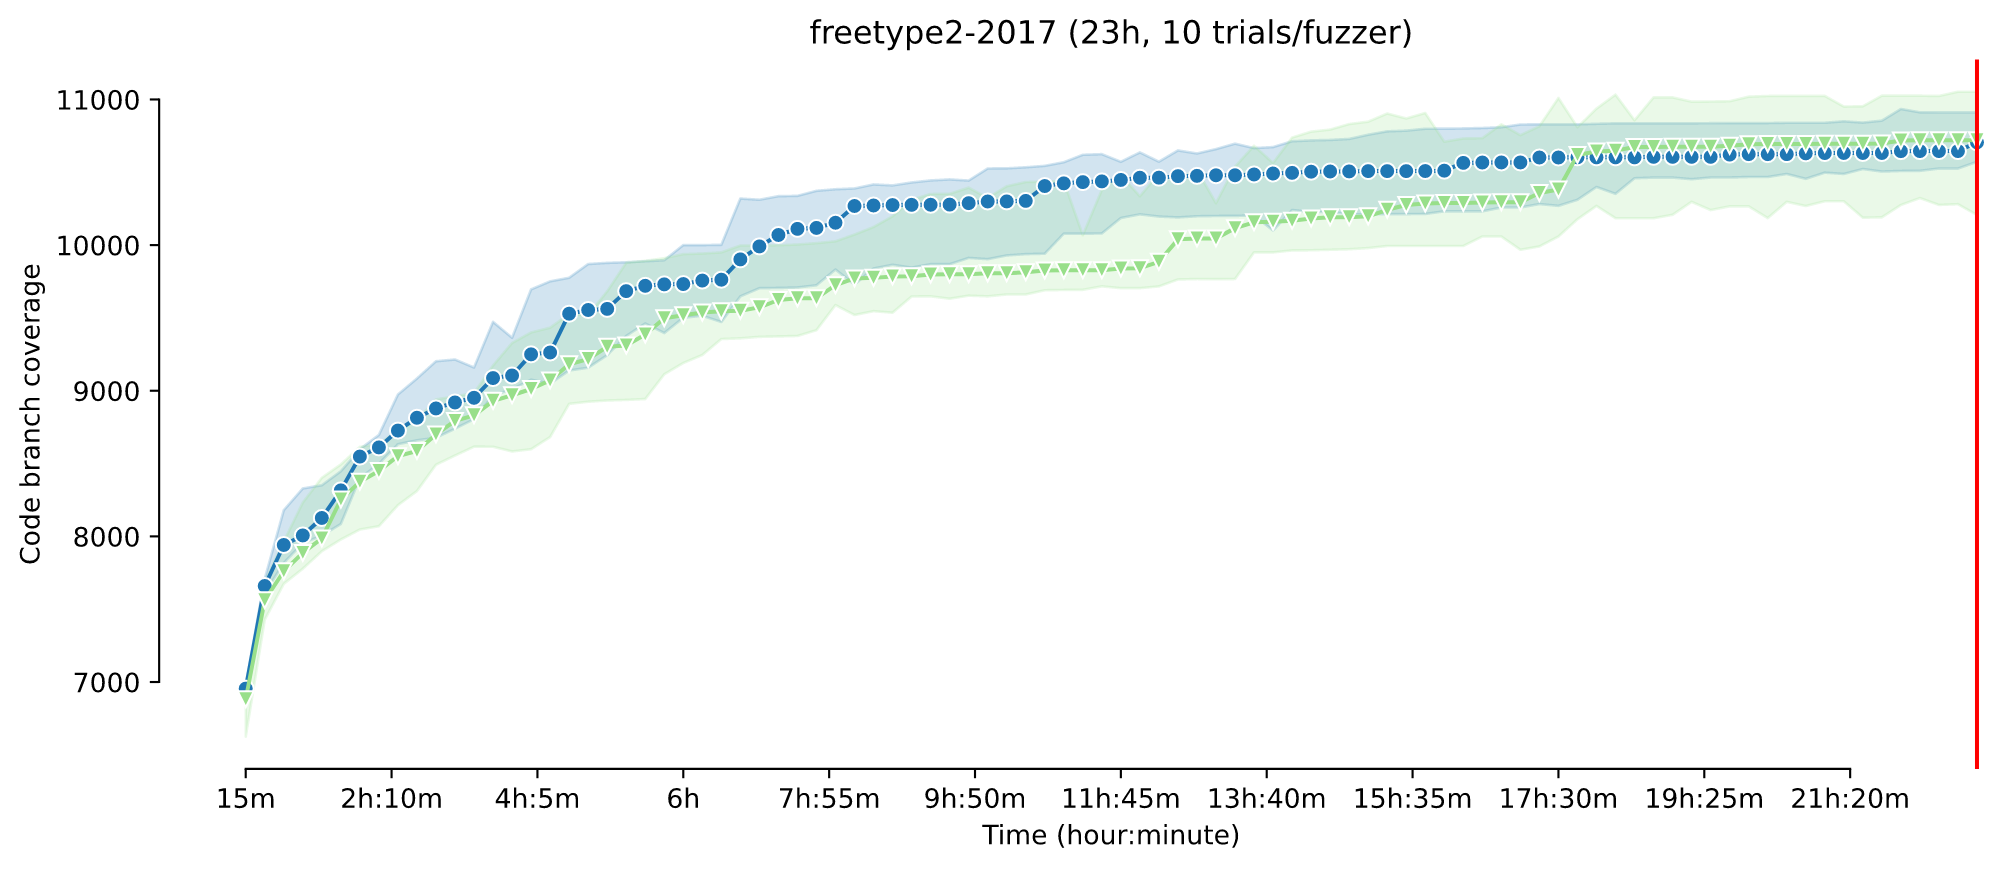
\includegraphics[width=0.65\textwidth]{assets/fuzzbench/symptr-25-1/freetype2-2017_coverage_growth.png}  & 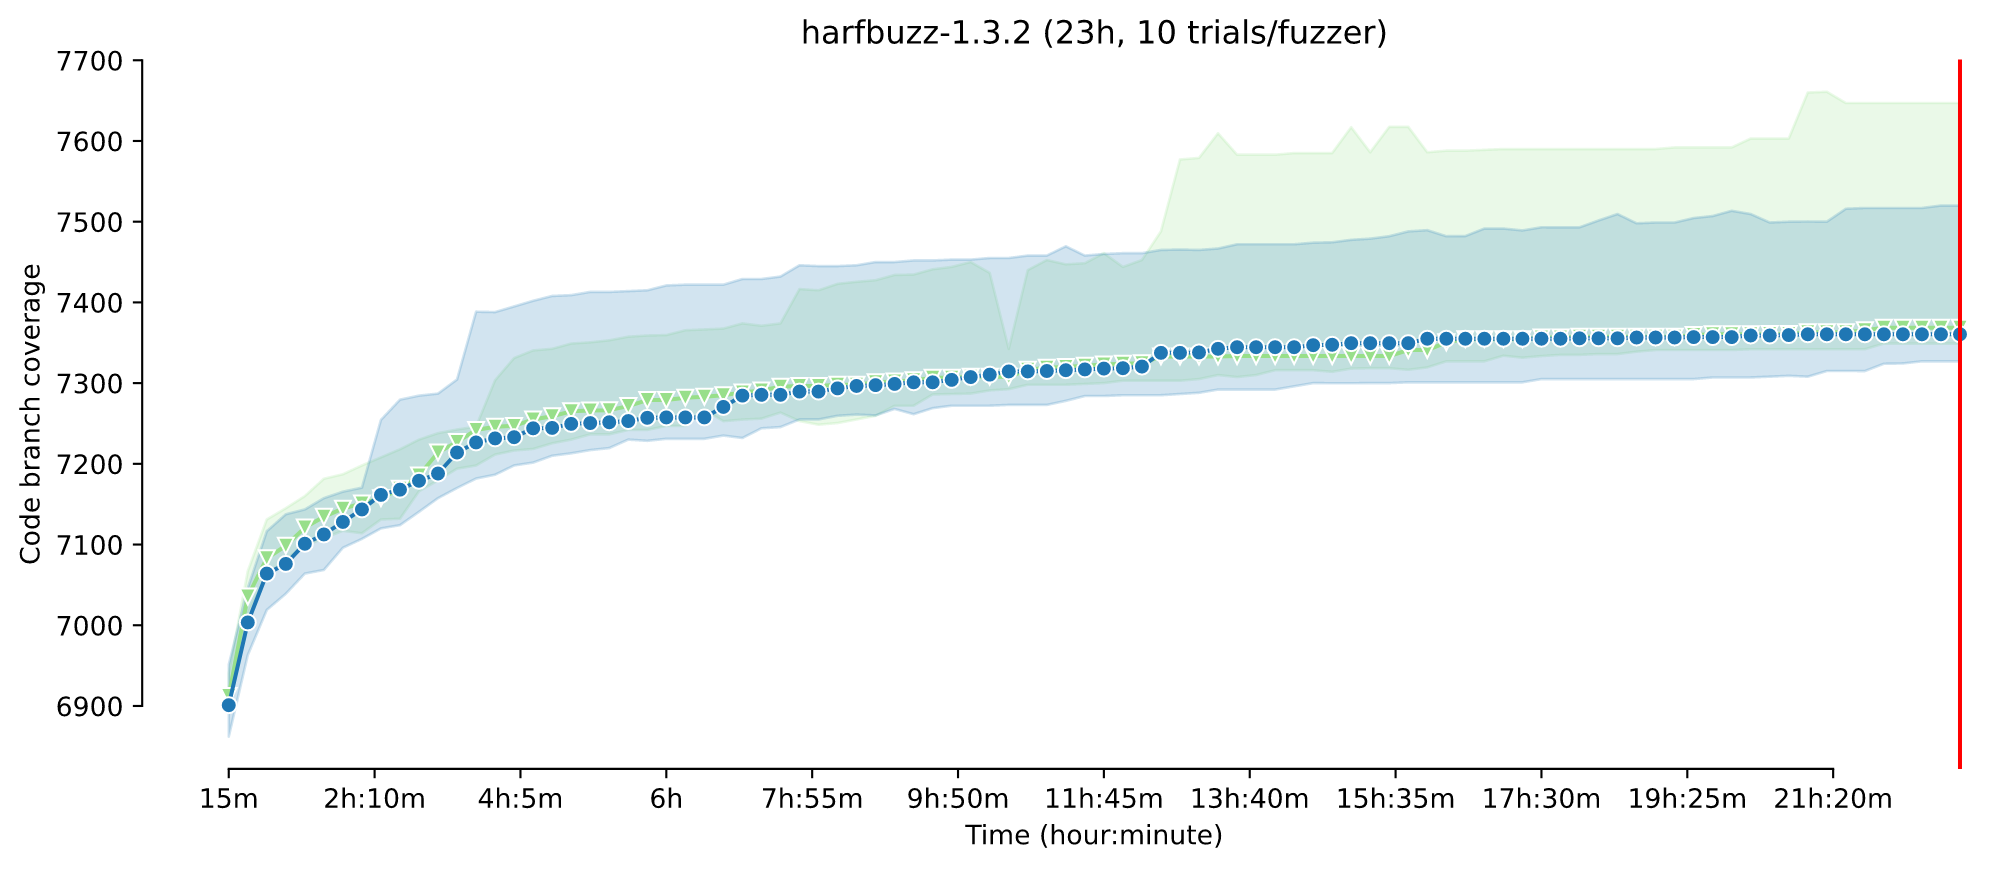
\includegraphics[width=0.65\textwidth]{assets/fuzzbench/symptr-25-1/harfbuzz-1.3.2_coverage_growth.png}        \\
            (a) freetype2                                                                                            & (b) harfbuzz                                                                                                   \\[6pt]
            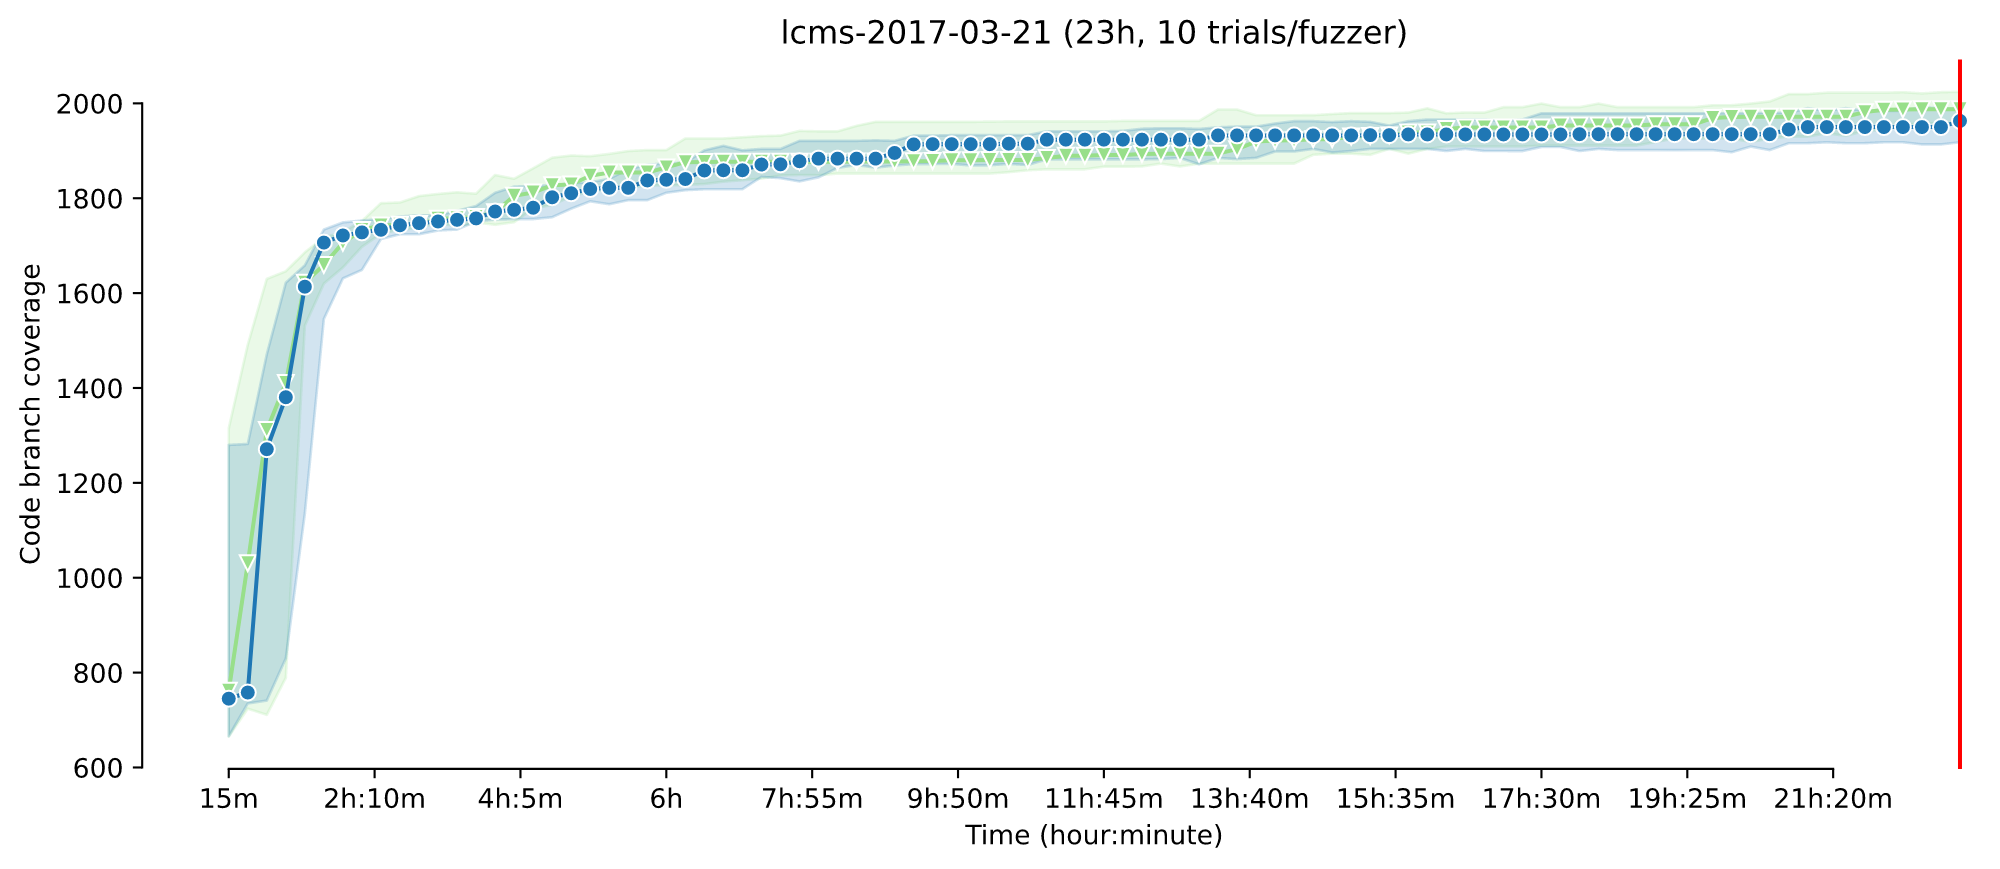
\includegraphics[width=0.65\textwidth]{assets/fuzzbench/symptr-25-1/lcms-2017-03-21_coverage_growth.png} & 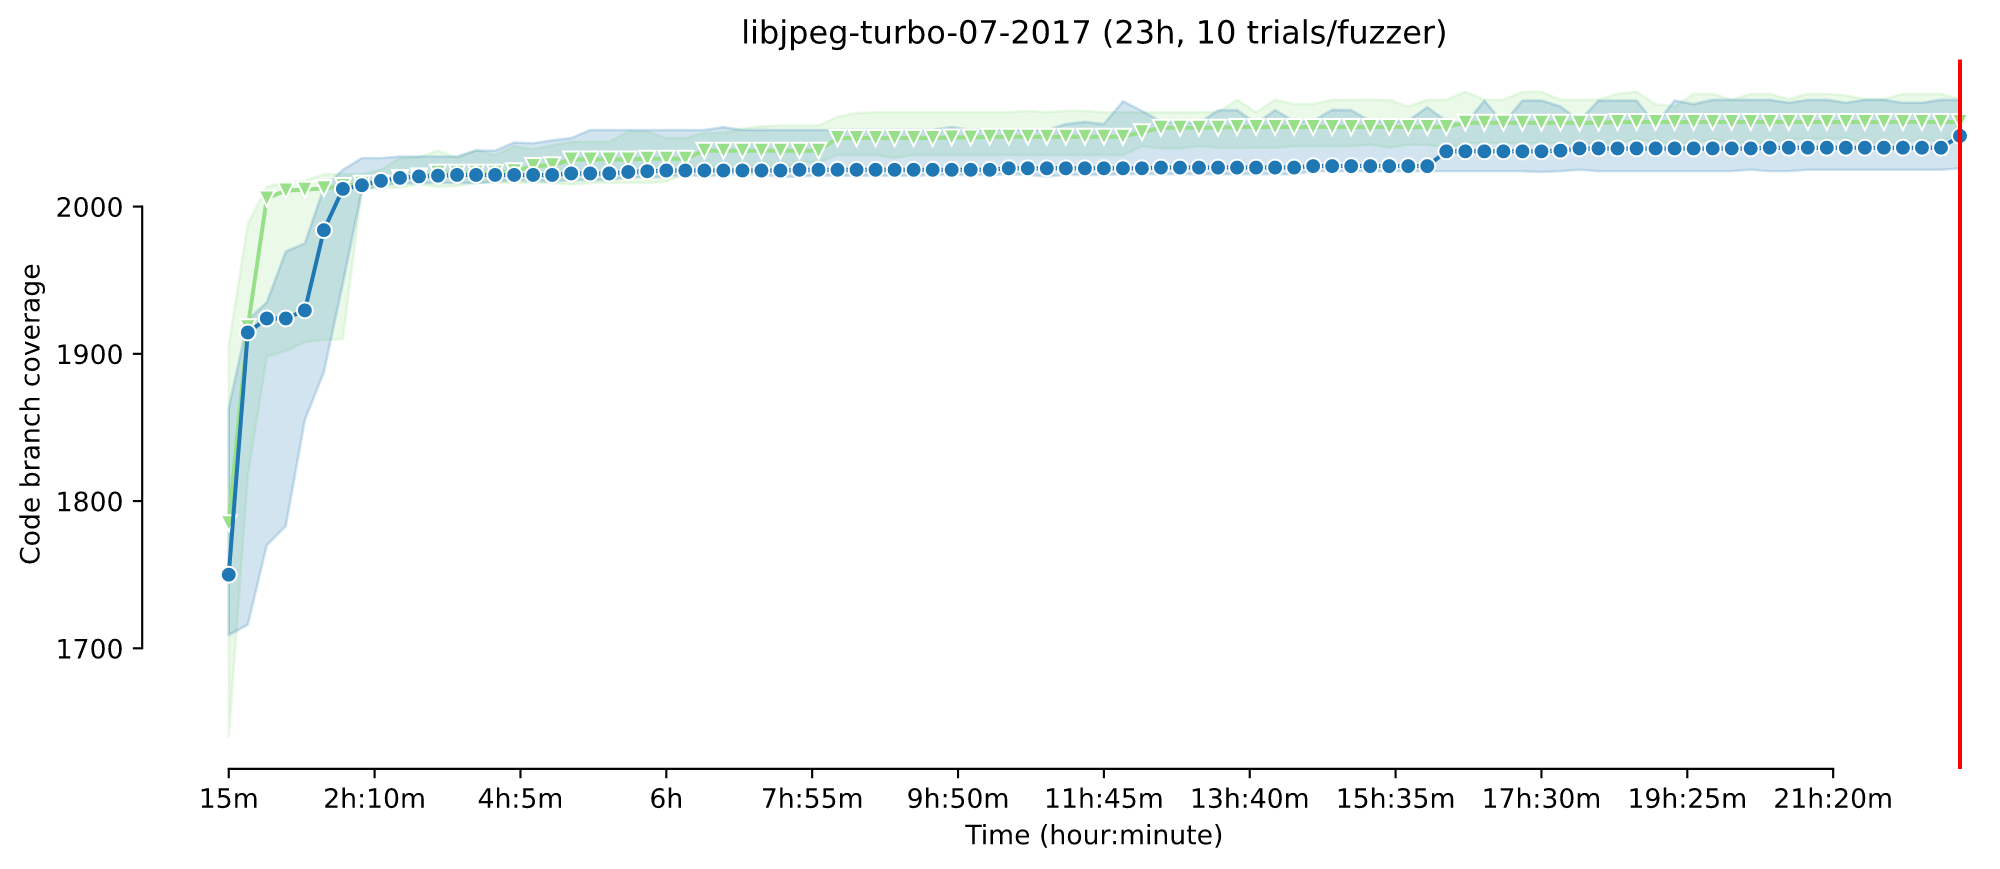
\includegraphics[width=0.65\textwidth]{assets/fuzzbench/symptr-25-1/libjpeg-turbo-07-2017_coverage_growth.png} \\
            (c) lcms                                                                                                 & (d) libjpeg                                                                                                    \\[6pt]
            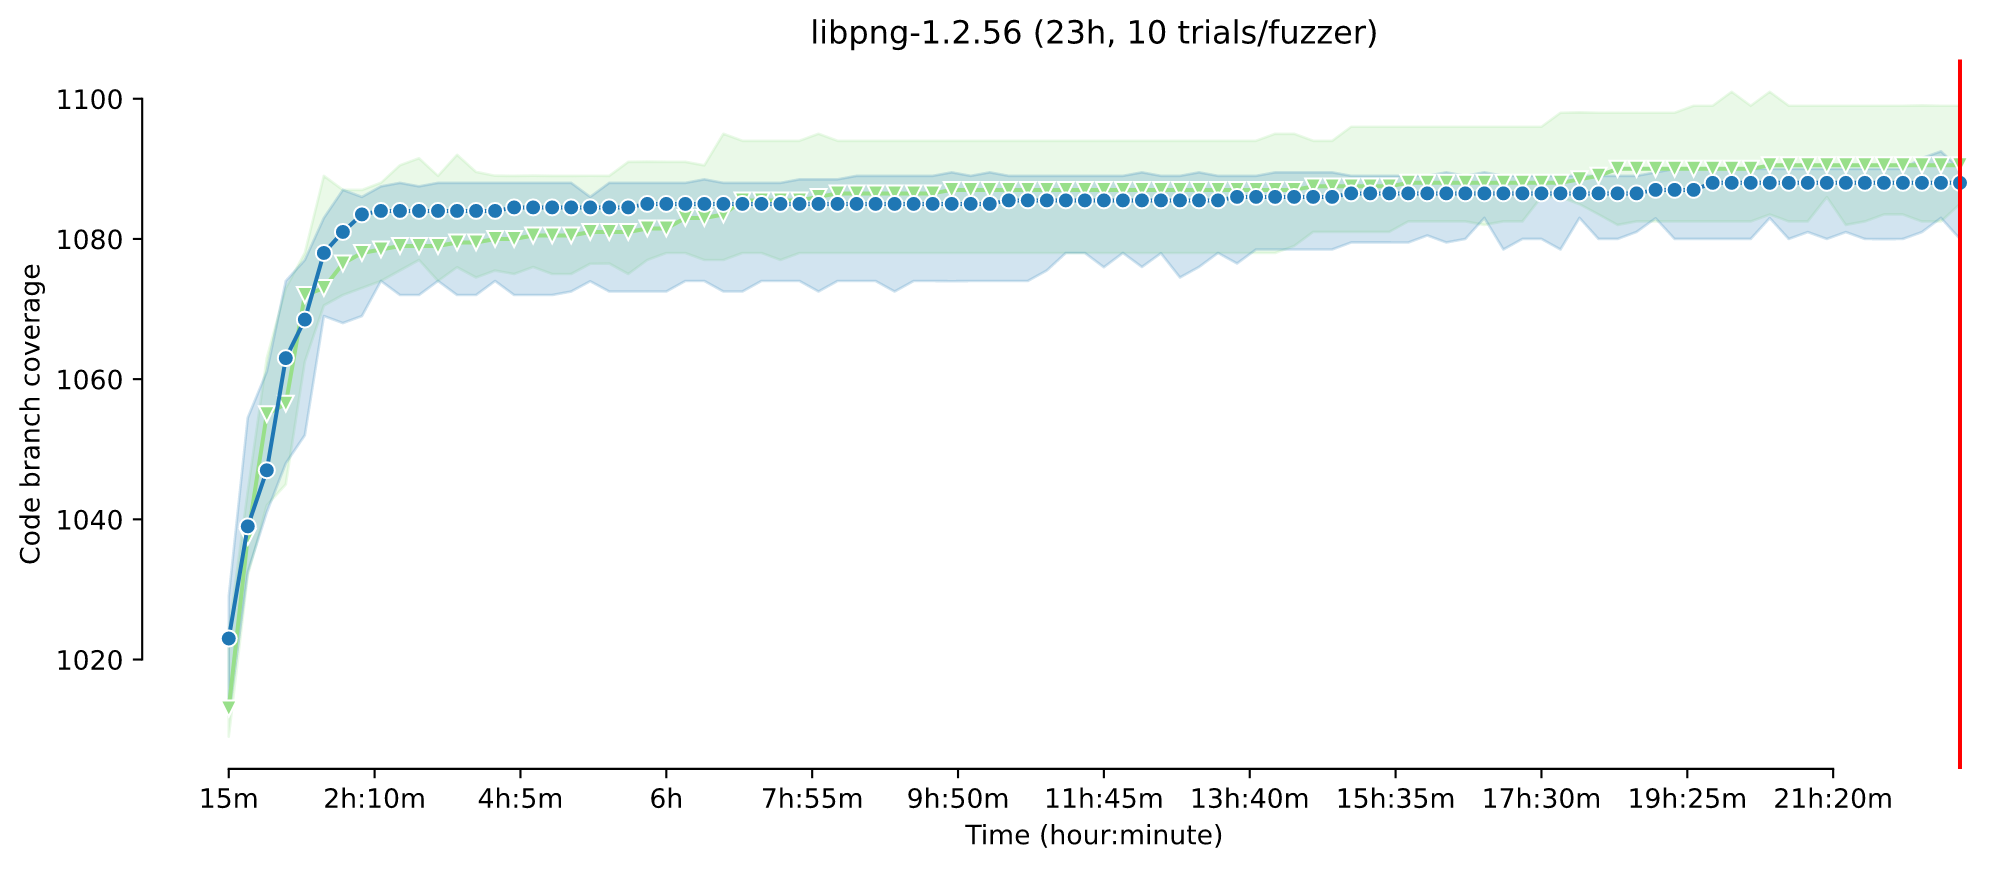
\includegraphics[width=0.65\textwidth]{assets/fuzzbench/symptr-25-1/libpng-1.2.56_coverage_growth.png}   & 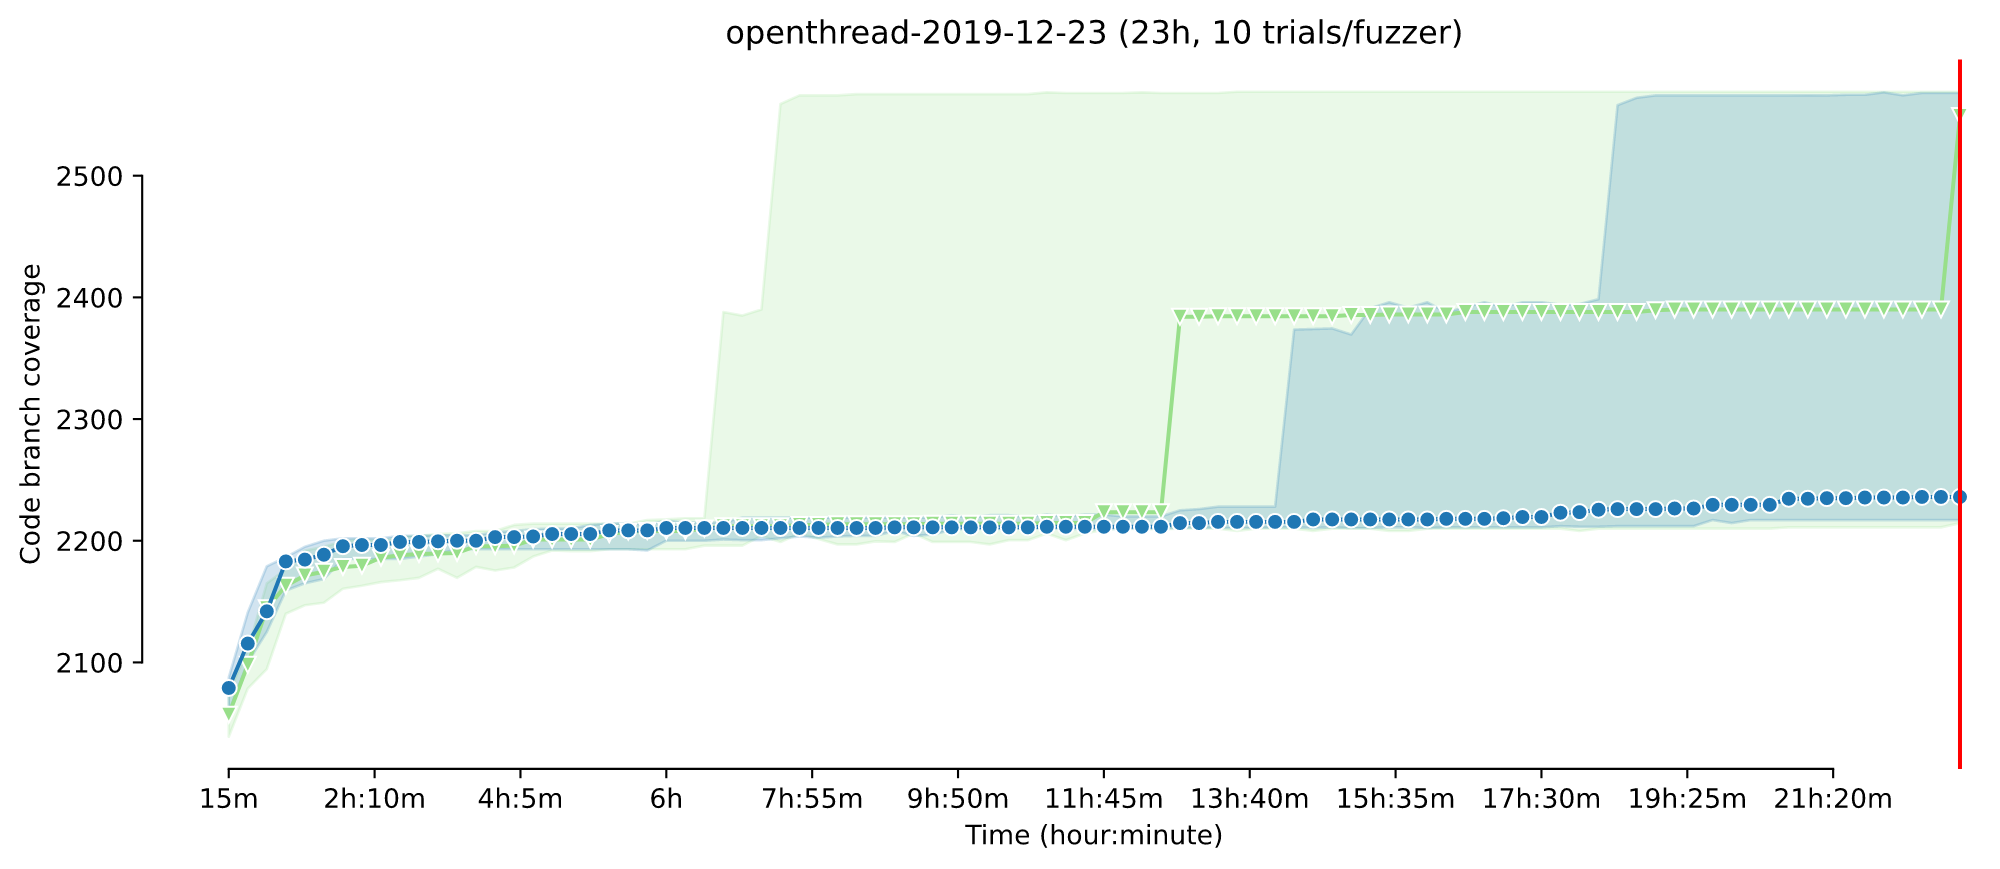
\includegraphics[width=0.65\textwidth]{assets/fuzzbench/symptr-25-1/openthread-2019-12-23_coverage_growth.png} \\
            (c) libpng                                                                                               & (d) openthread                                                                                                 \\[6pt]
            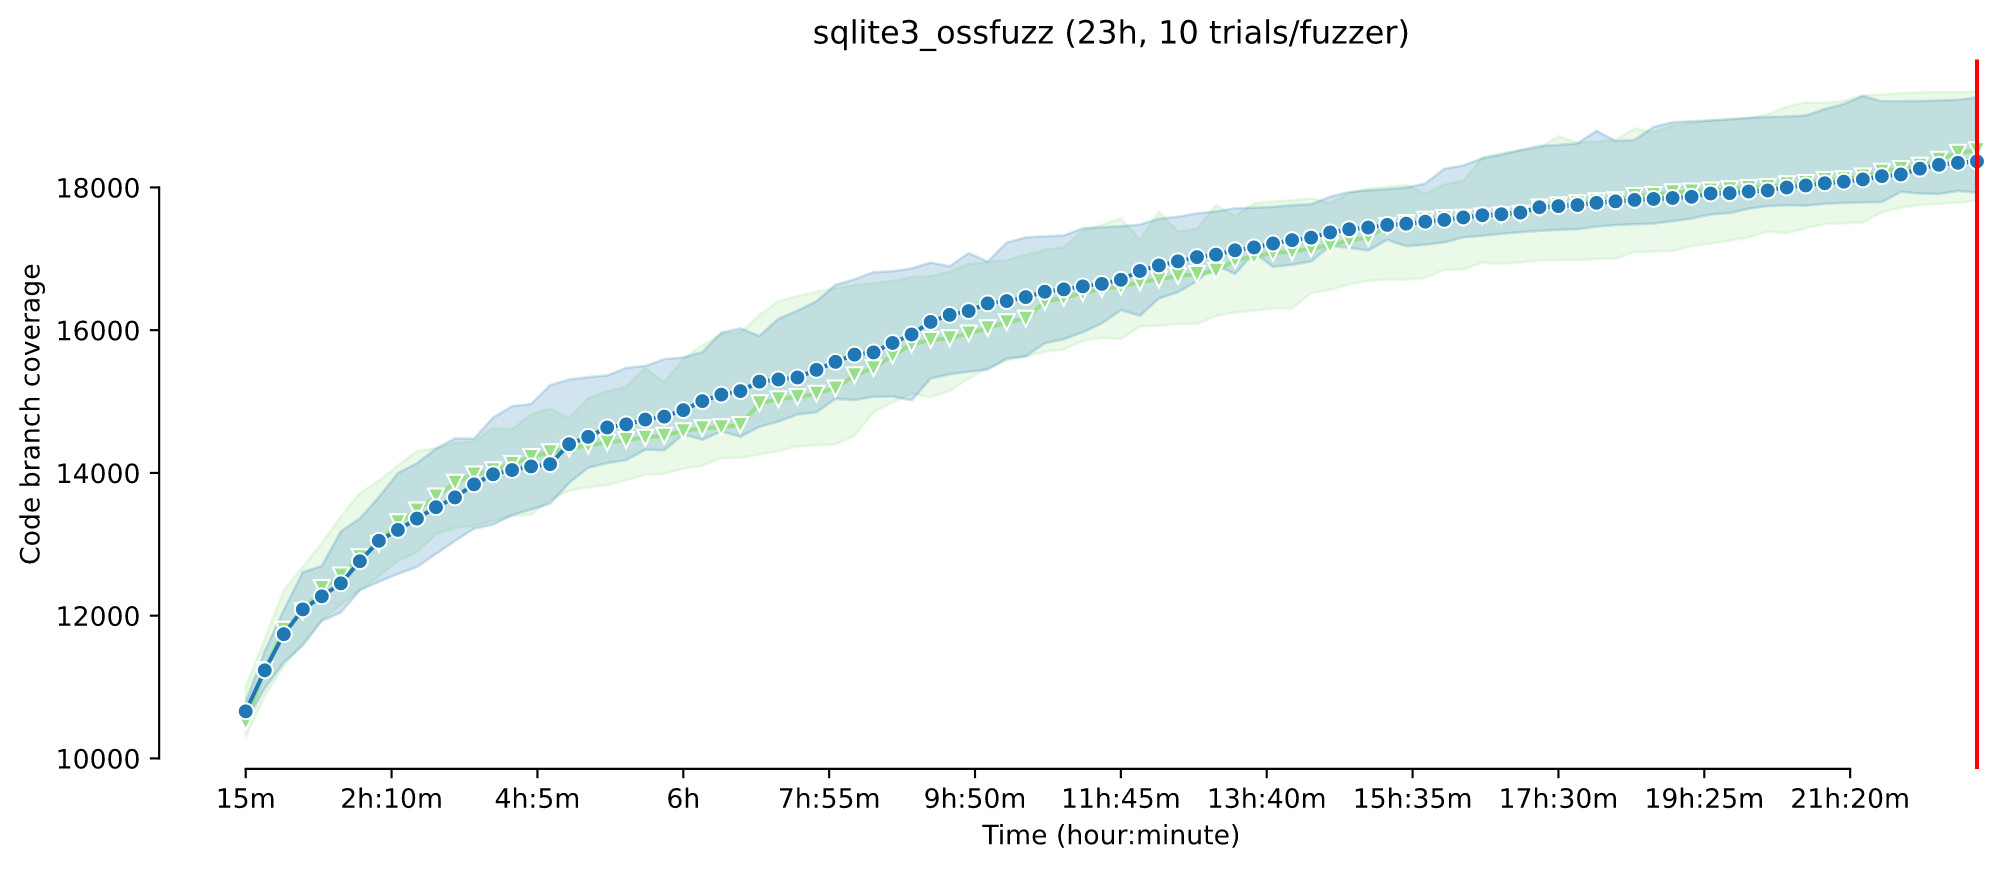
\includegraphics[width=0.65\textwidth]{assets/fuzzbench/symptr-25-1/sqlite3_ossfuzz_coverage_growth.png} & \includegraphics[width=0.65\textwidth]{assets/fuzzbench/symptr-25-1/fuzzbench-legend.png}                      \\
            (c) sqlite3                                                                                              & (d) legend                                                                                                     \\[6pt]
        \end{tabular}
    }
    \caption{Fuzzbench: Symptr-25-1 coverage growth.}
    \label{fig:fuzzbench:symptr-25-1}
\end{figure}

\begin{figure}[b]
    \centering
    \resizebox{\columnwidth}{!}{%
        \begin{tabular}{cc}
            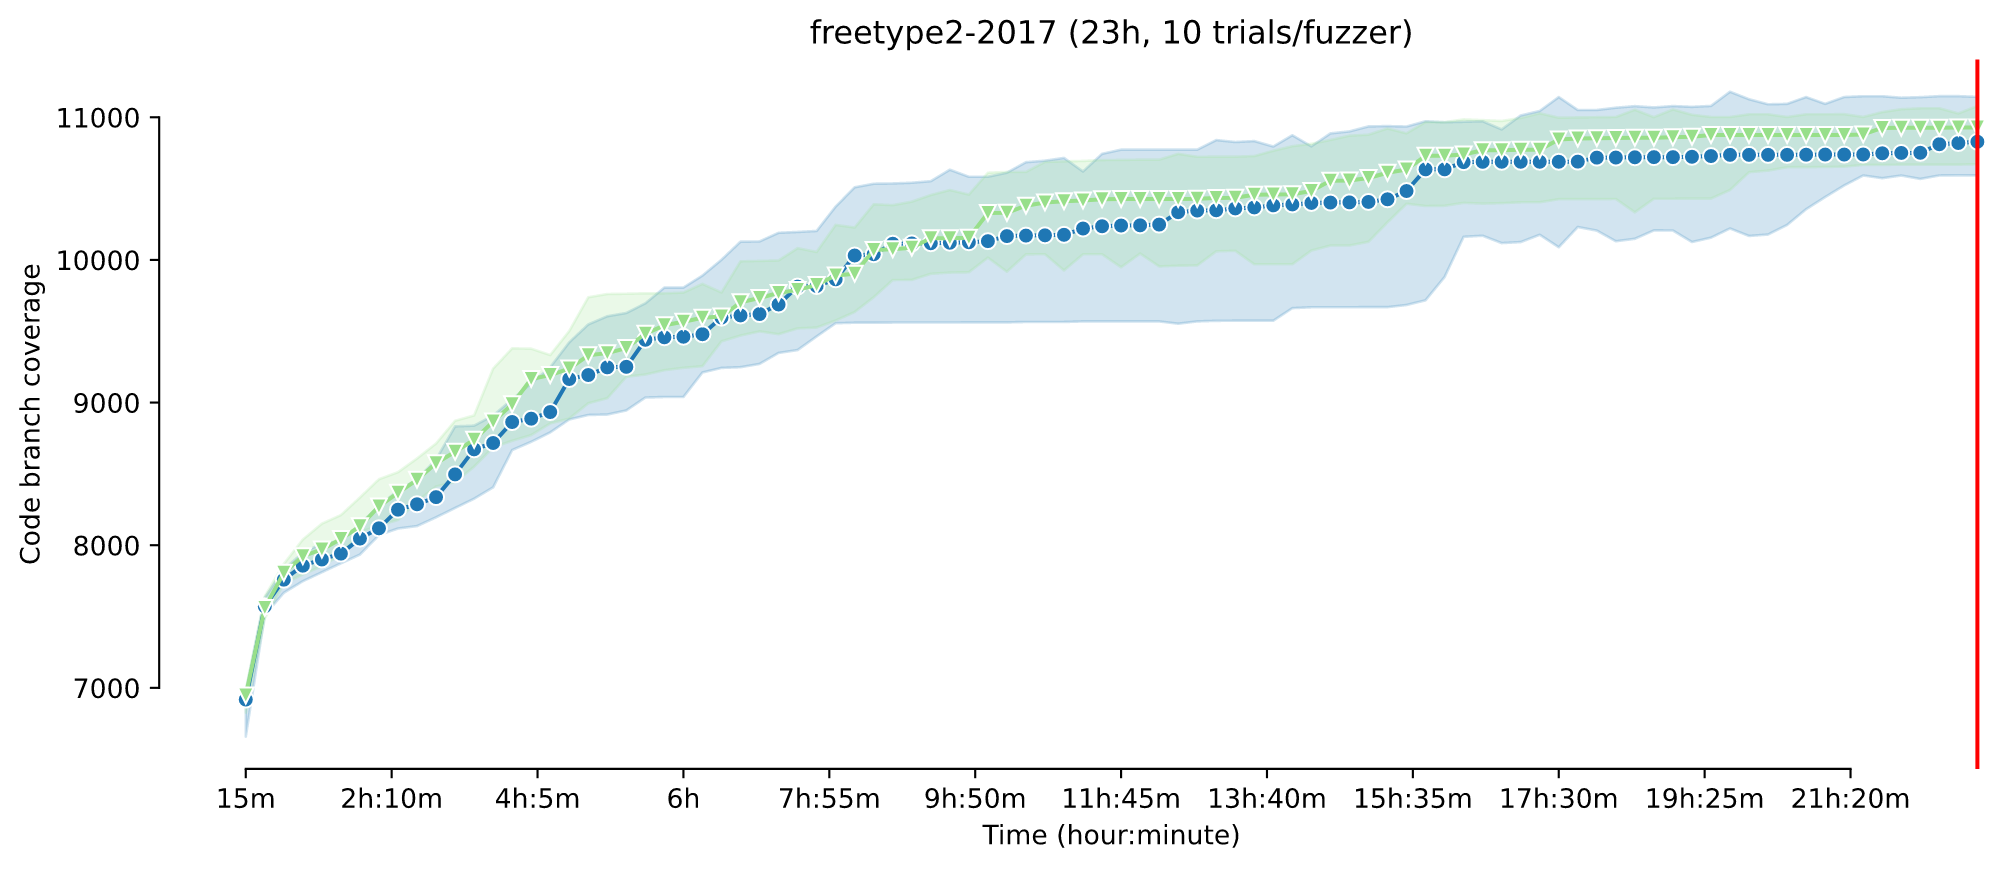
\includegraphics[width=0.65\textwidth]{assets/fuzzbench/symptr-25-vs-35-2/freetype2-2017_coverage_growth.png}  & 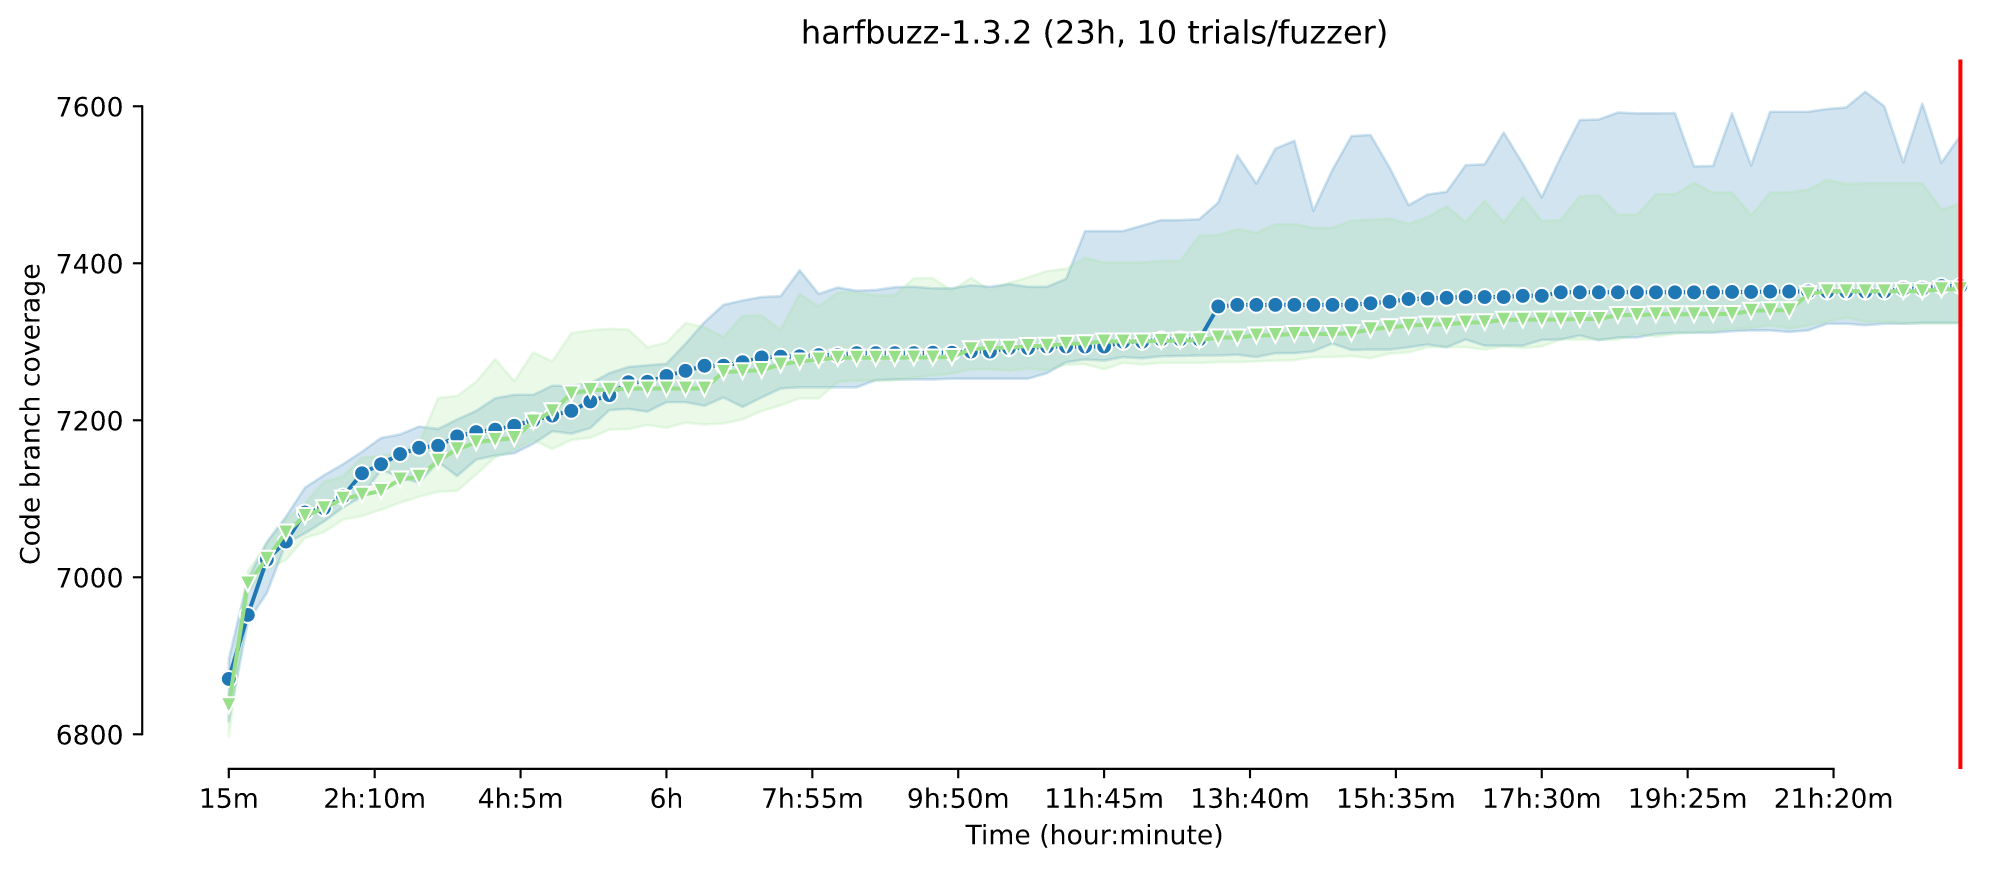
\includegraphics[width=0.65\textwidth]{assets/fuzzbench/symptr-25-vs-35-2/harfbuzz-1.3.2_coverage_growth.png}        \\
            (a) freetype2                                                                                                  & (b) harfbuzz                                                                                                         \\[6pt]
            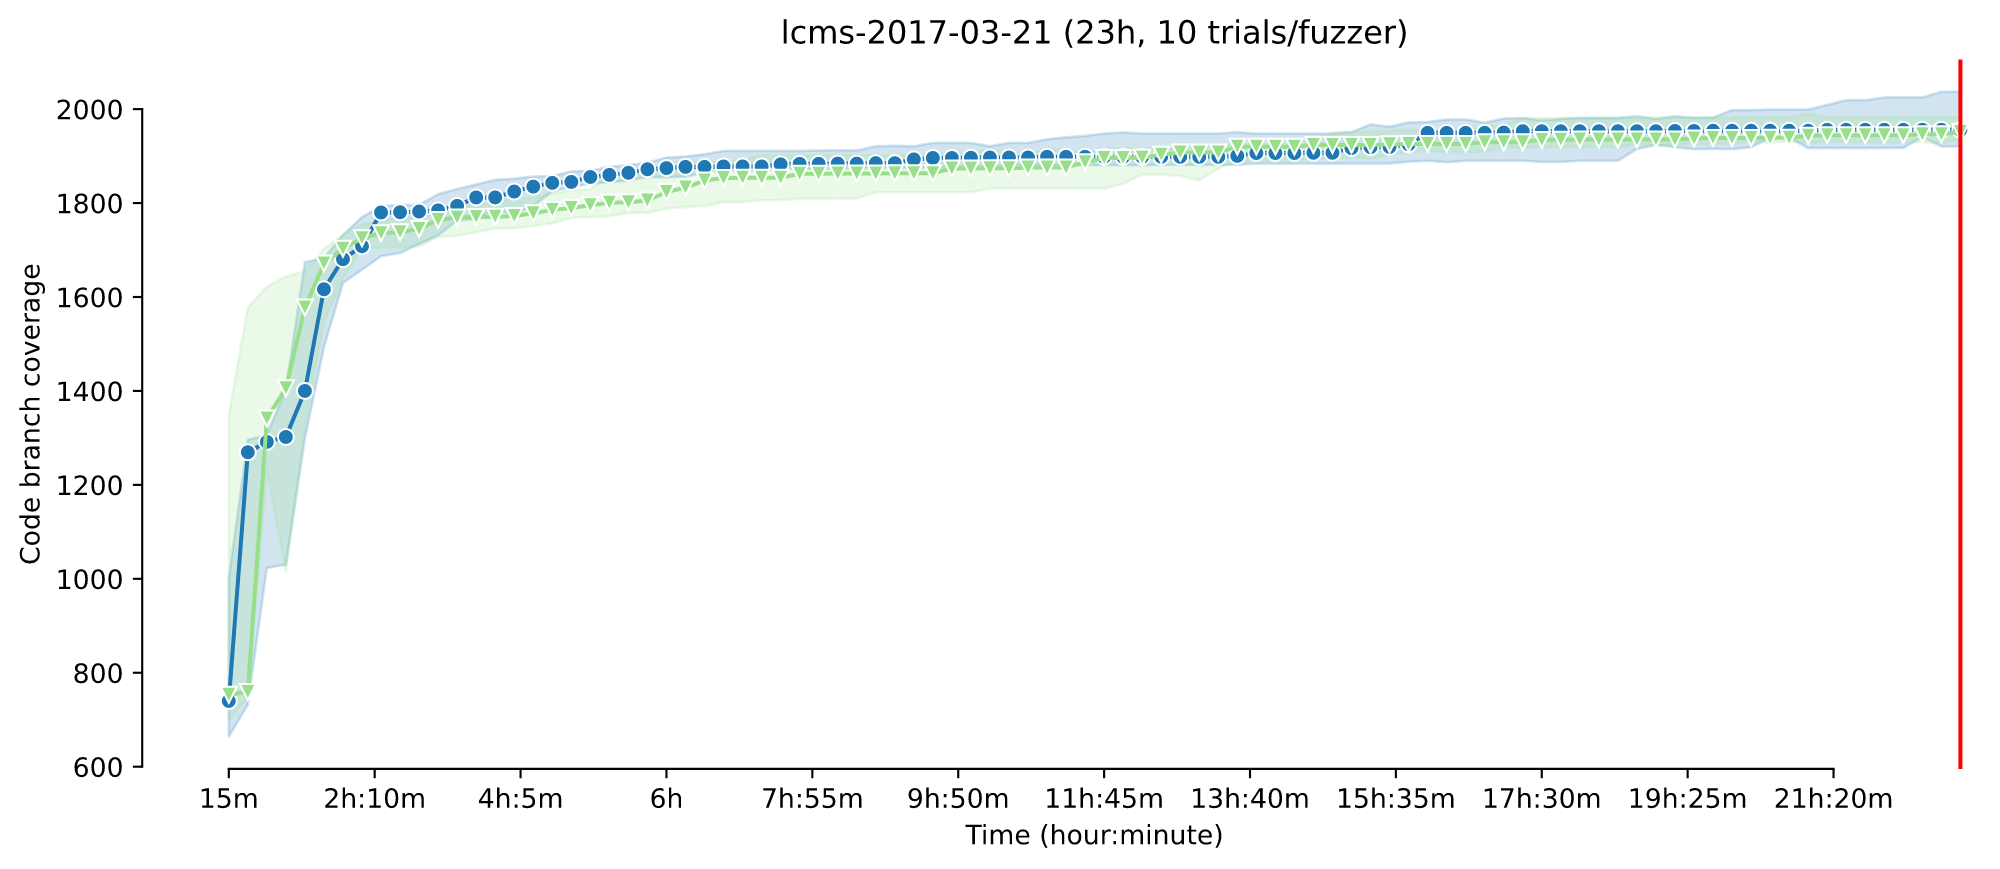
\includegraphics[width=0.65\textwidth]{assets/fuzzbench/symptr-25-vs-35-2/lcms-2017-03-21_coverage_growth.png} & 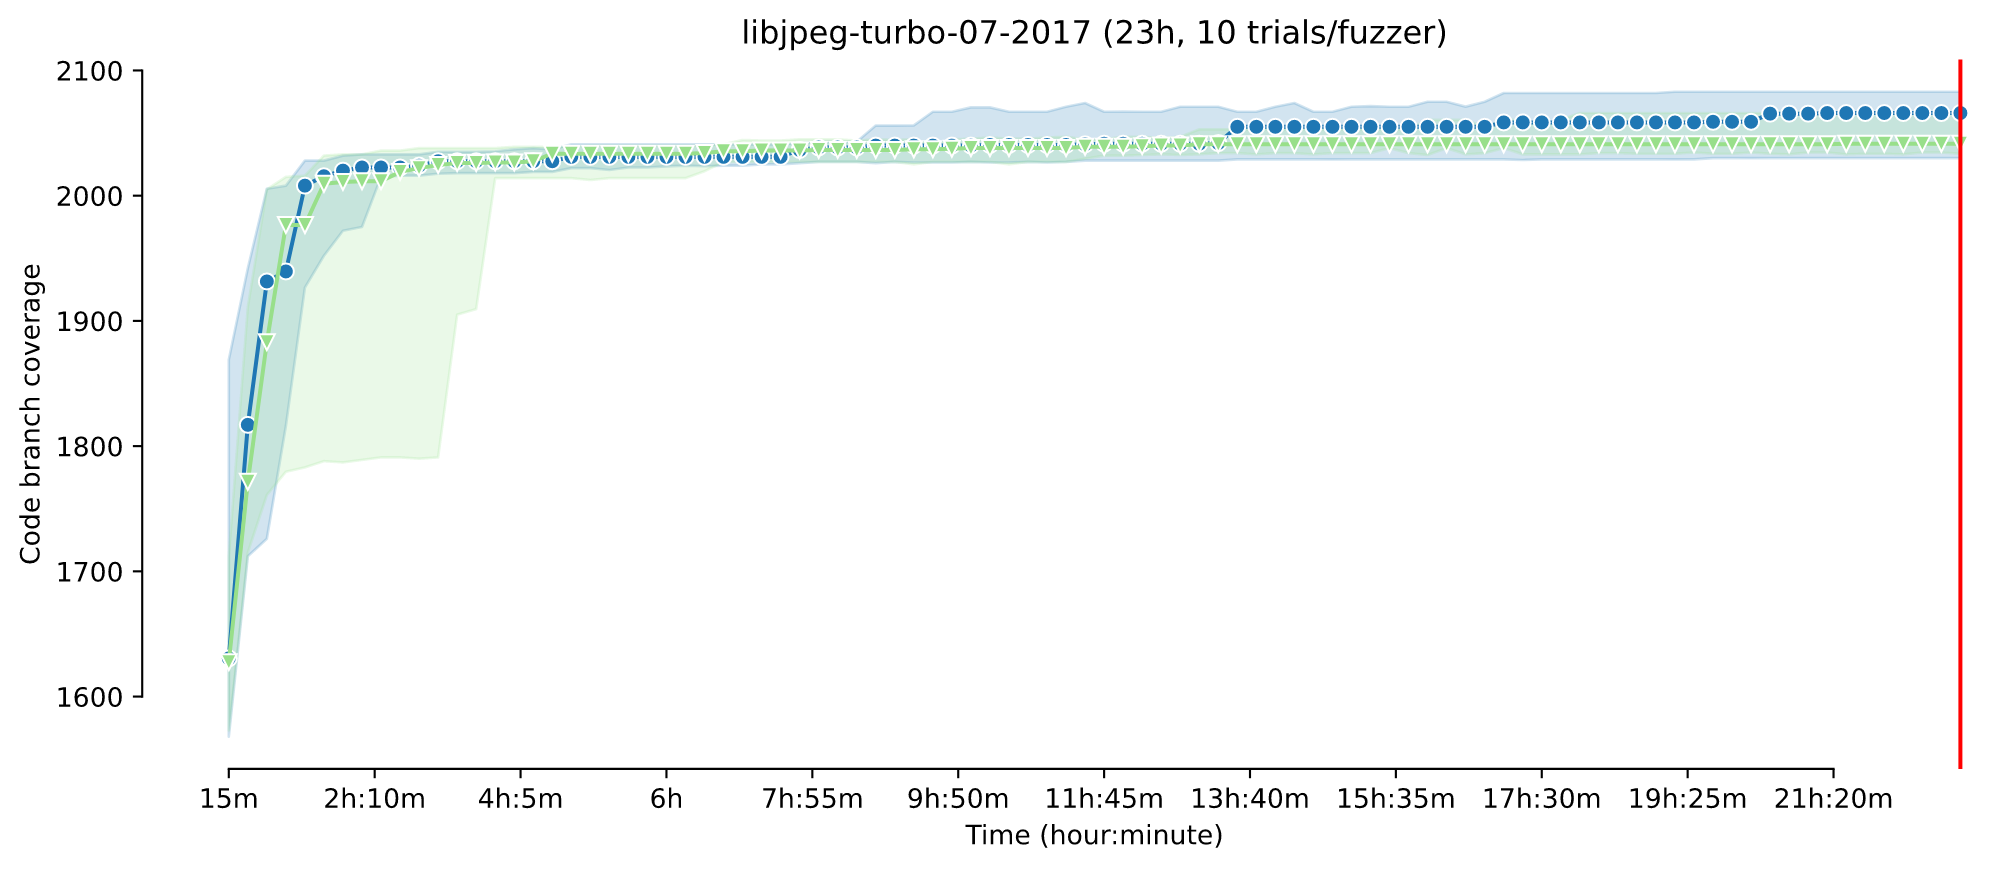
\includegraphics[width=0.65\textwidth]{assets/fuzzbench/symptr-25-vs-35-2/libjpeg-turbo-07-2017_coverage_growth.png} \\
            (c) lcms                                                                                                       & (d) libjpeg                                                                                                          \\[6pt]
            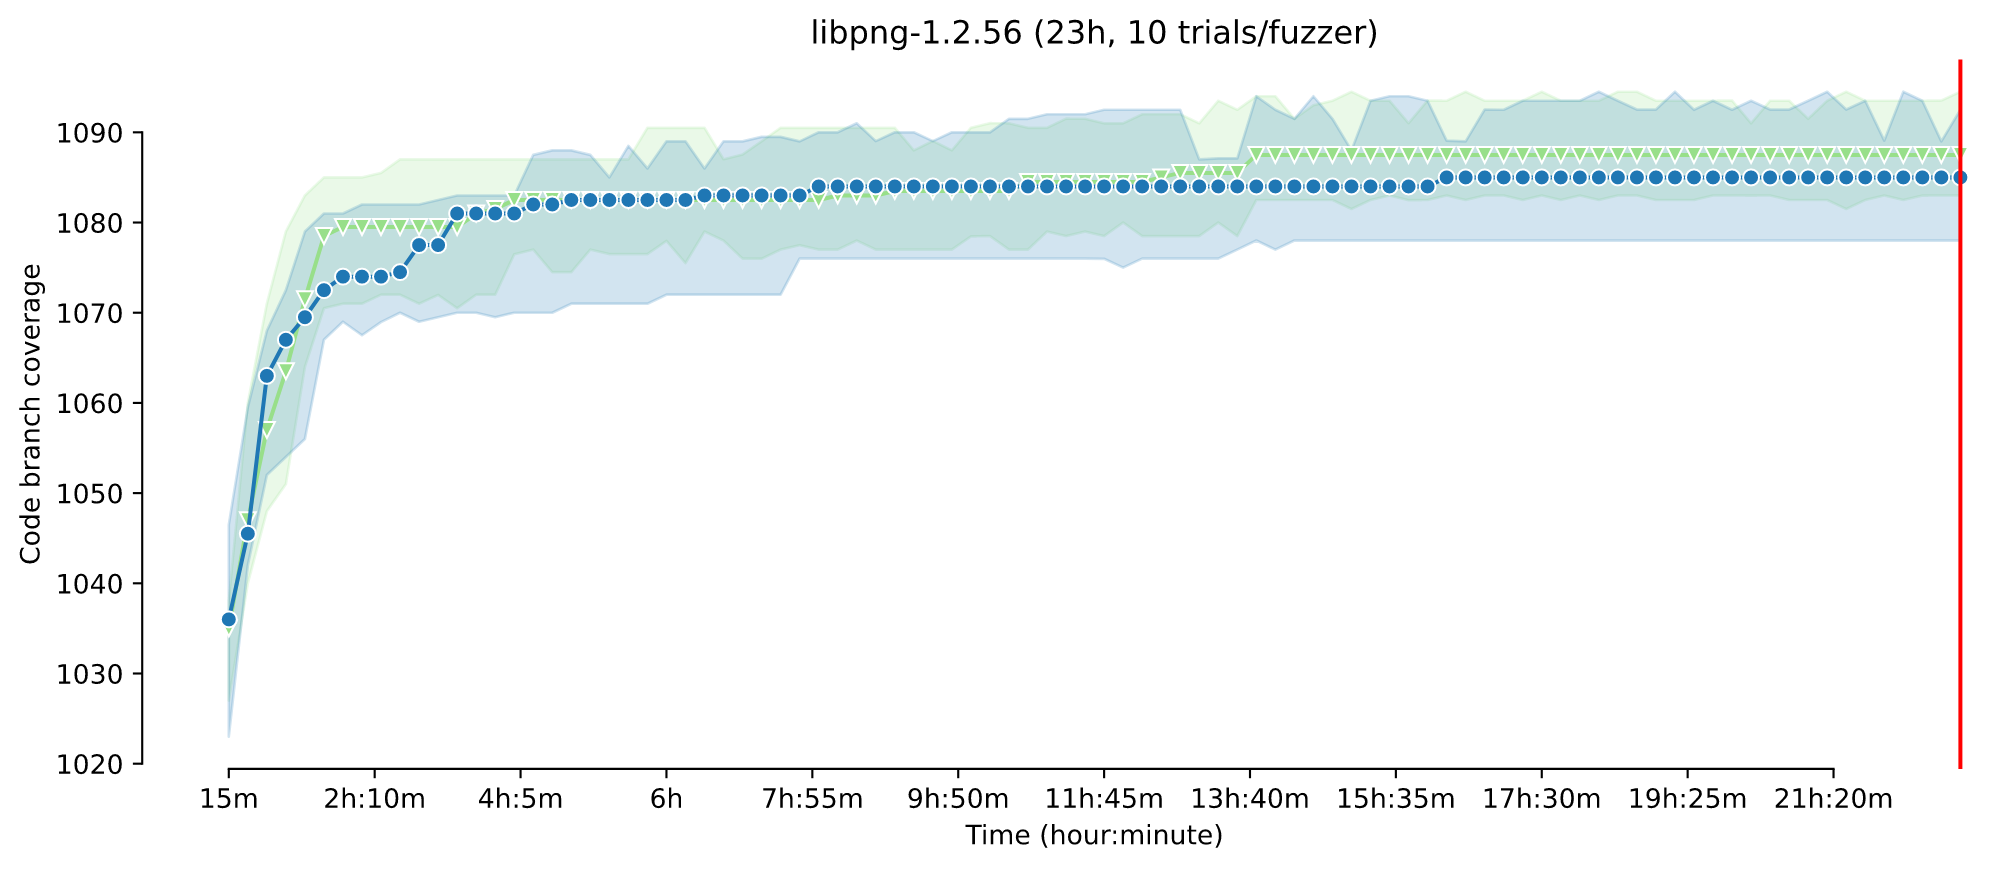
\includegraphics[width=0.65\textwidth]{assets/fuzzbench/symptr-25-vs-35-2/libpng-1.2.56_coverage_growth.png}   & 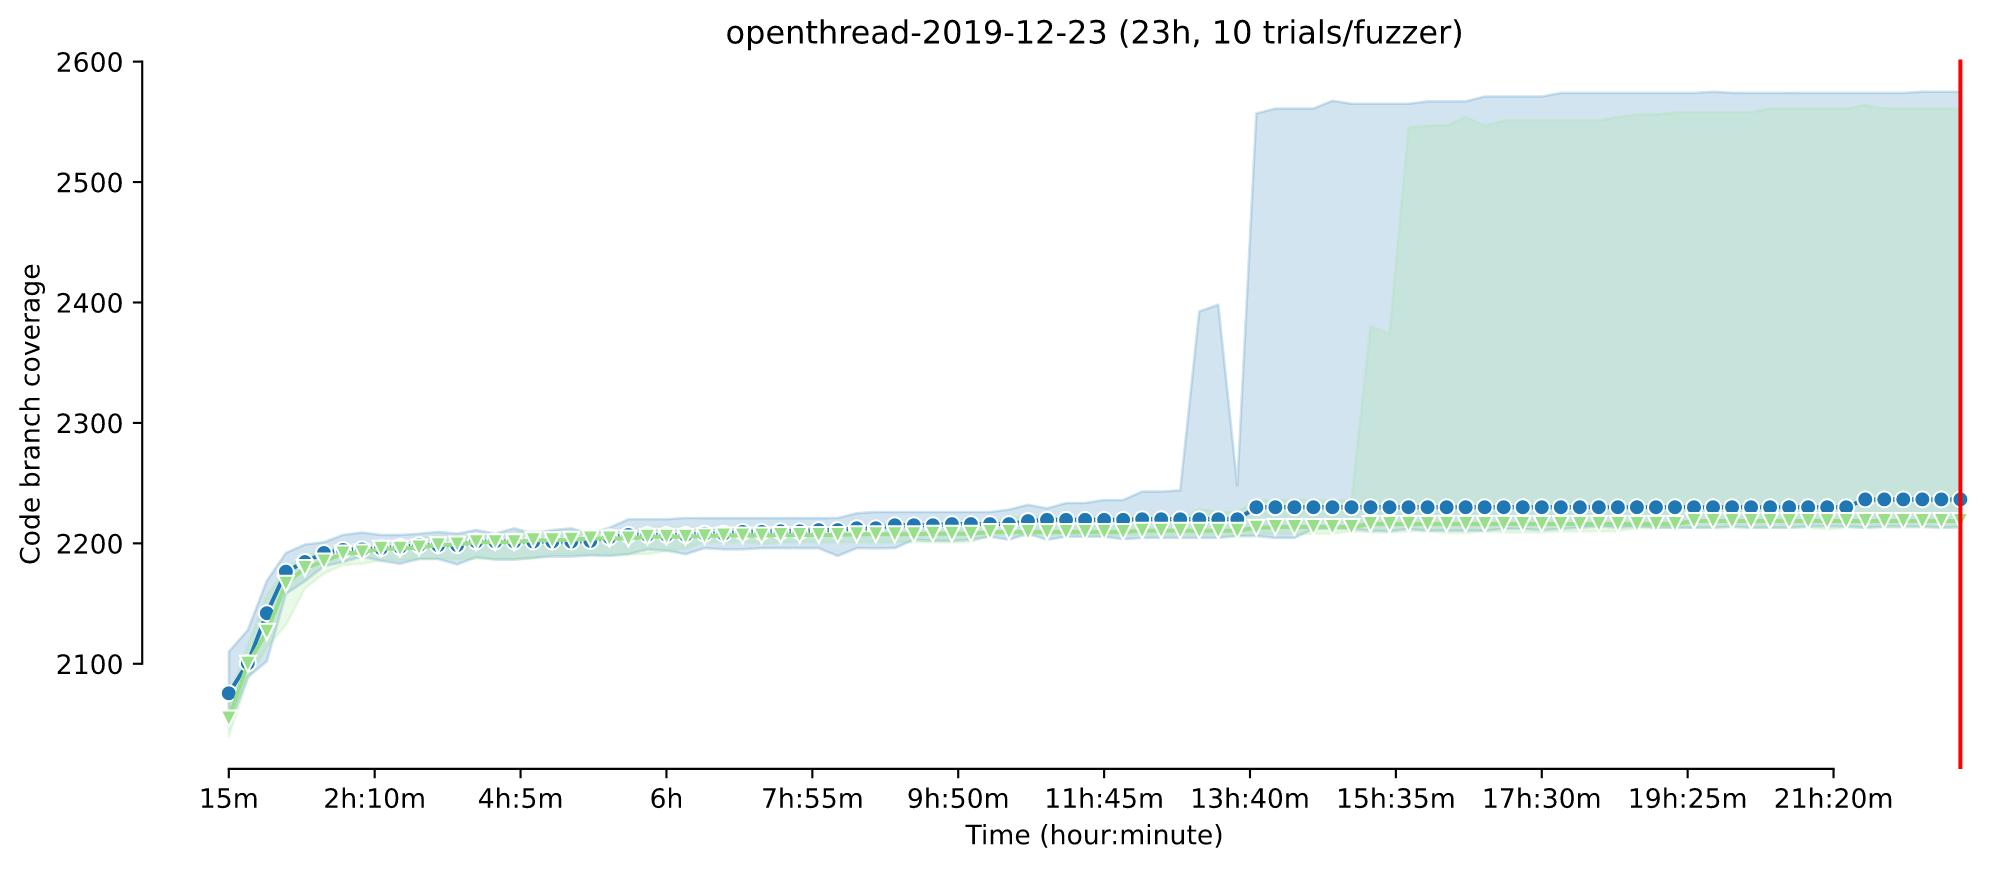
\includegraphics[width=0.65\textwidth]{assets/fuzzbench/symptr-25-vs-35-2/openthread-2019-12-23_coverage_growth.png} \\
            (c) libpng                                                                                                     & (d) openthread                                                                                                       \\[6pt]
            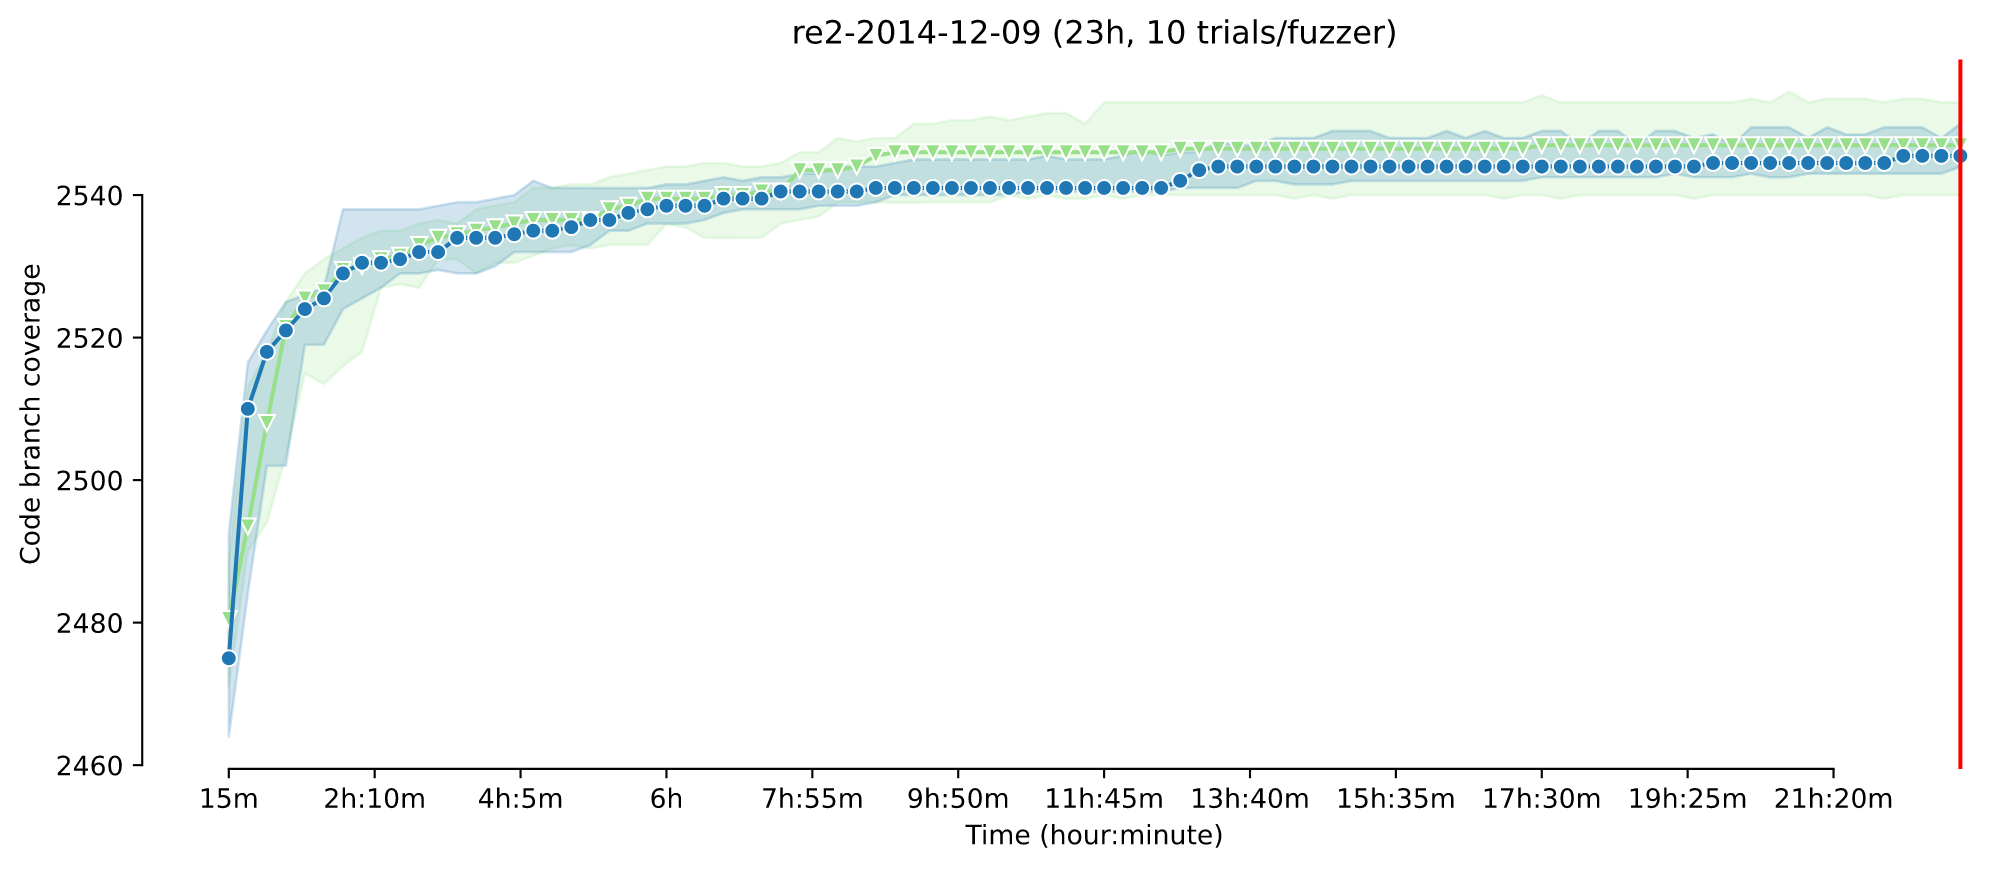
\includegraphics[width=0.65\textwidth]{assets/fuzzbench/symptr-25-vs-35-2/re2-2014-12-09_coverage_growth.png}  & 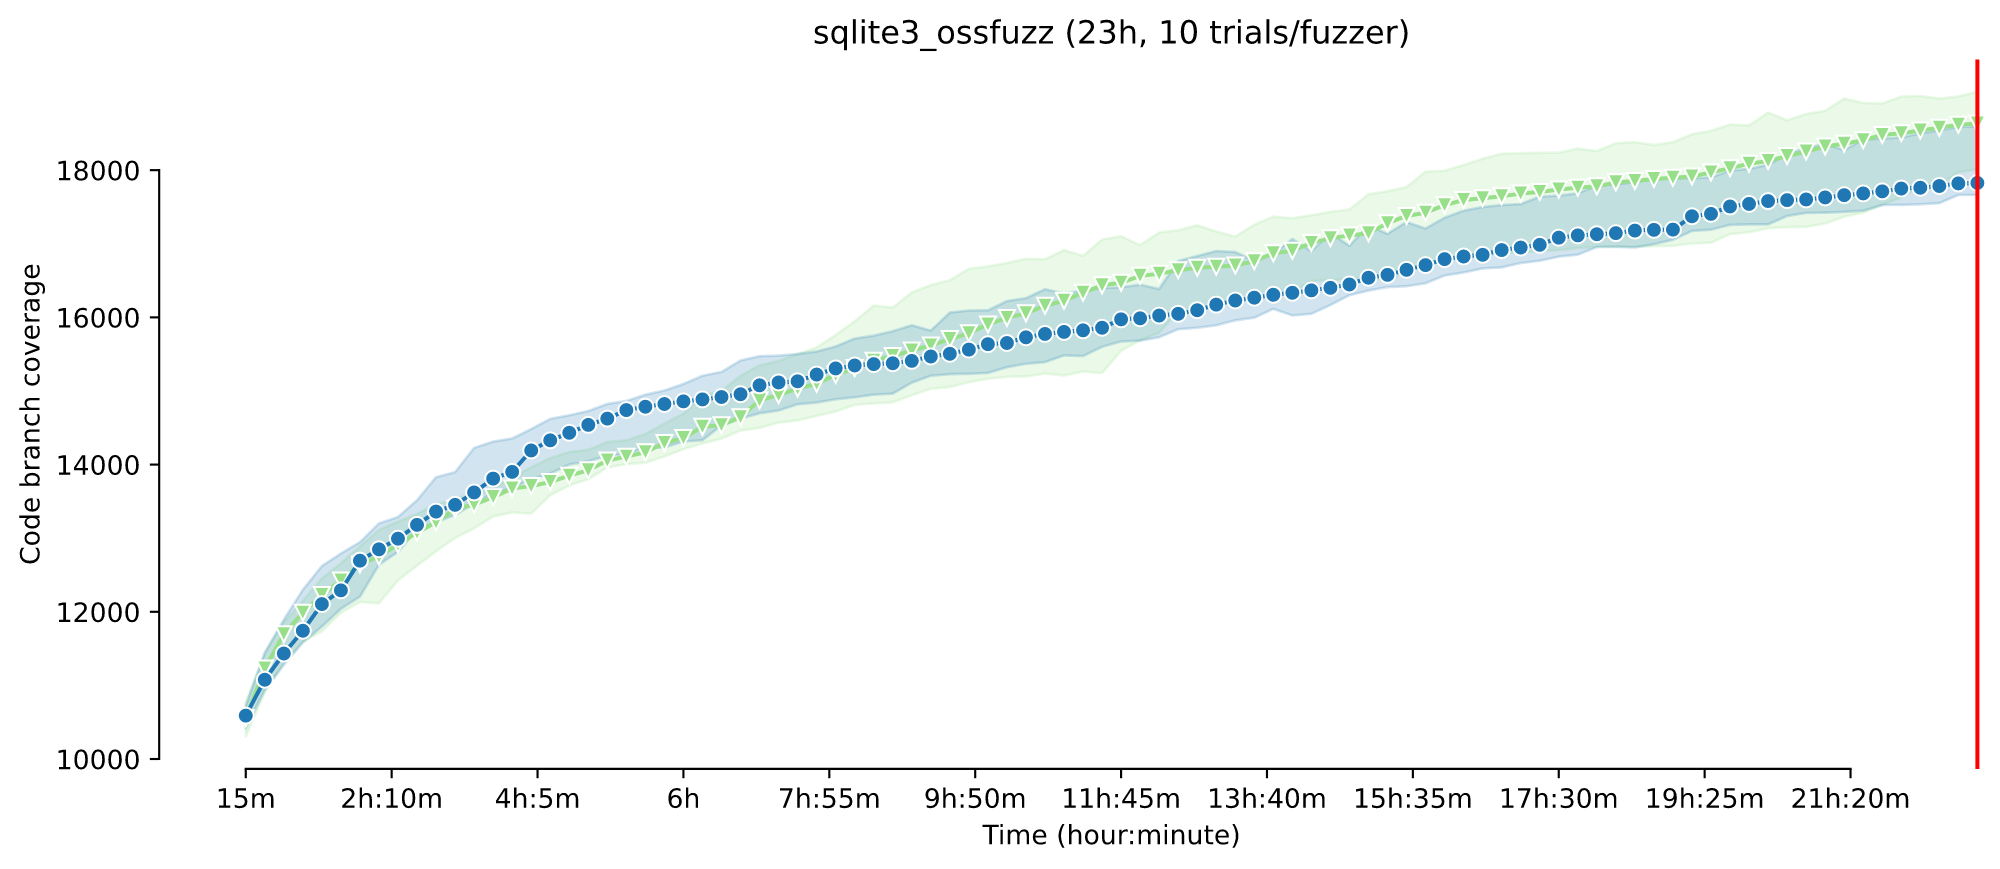
\includegraphics[width=0.65\textwidth]{assets/fuzzbench/symptr-25-vs-35-2/sqlite3_ossfuzz_coverage_growth.png}       \\
            (c) re2                                                                                                        & (d) sqlite3                                                                                                          \\[6pt]
            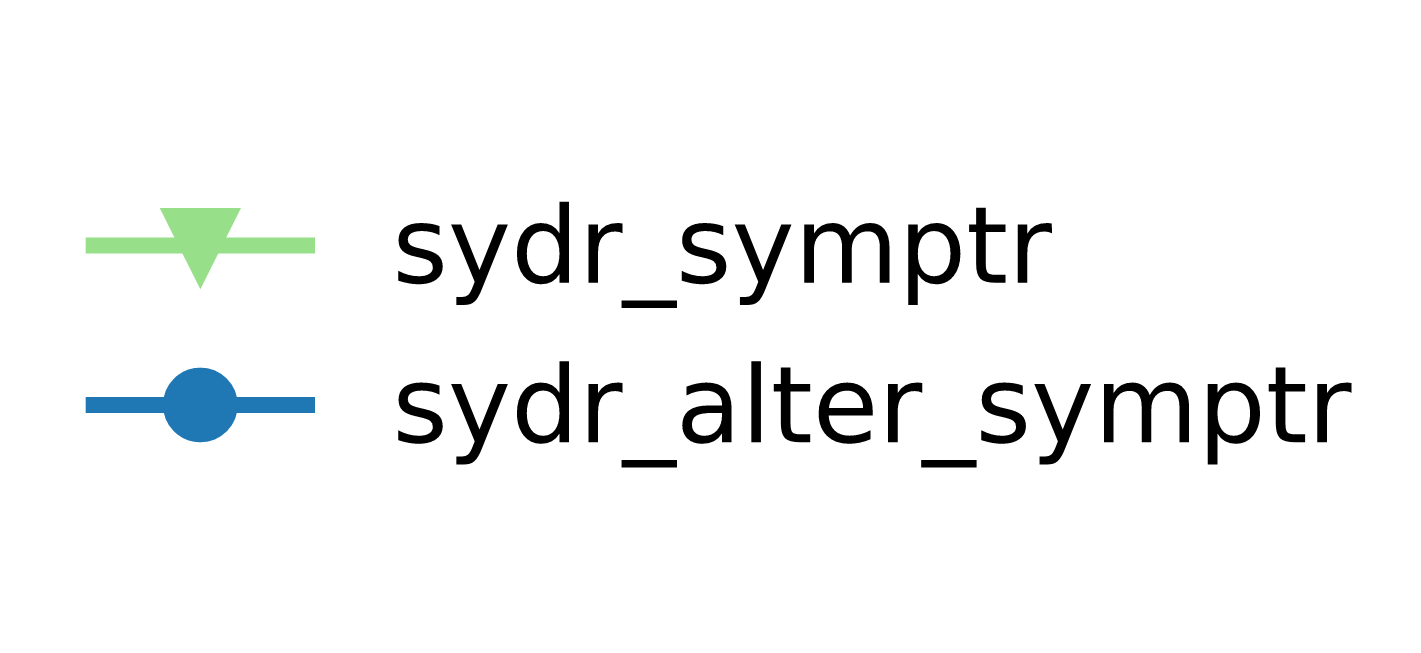
\includegraphics[width=0.65\textwidth]{assets/fuzzbench/symptr-25-vs-35-2/fuzzbench-legend.png}                &                                                                                                                      \\
            (c) legend                                                                                                     &                                                                                                                      \\[6pt]
        \end{tabular}
    }
    \caption{Fuzzbench: Symptr-25-vs-35-2 coverage growth.}
    \label{fig:fuzzbench:symptr-25-vs-35-2}
\end{figure}

